%
% ADA NOTES
%
\documentclass[a4paper,11pt,twoside]{article}
\usepackage{graphicx}

% Add mystyle.sty
\usepackage{mystyle}
\usepackage{amsmath}
\usepackage{amsfonts}

\begin{document}%%%% DOCUMENT %%%%

% !TEX root = ../notes.tex

\begin{titlepage} %Titre
\begin{center}
\newcommand{\HRule}{\rule{\linewidth}{0.5mm}} % Defines a new command for the horizontal lines, change thickness here
\center % Center everything on the page
 
 
 %----------------------------------------------------------------------------------------
% TITLE SECTION
%----------------------------------------------------------------------------------------




\begin{figure} [h] %----------- SubGraph ---------------------
\centerline{
\subfigure{
\includegraphics[height = 2 cm]{./pic/EPFL.png}  }
\subfigure{
\includegraphics[height = 2 cm]{./pic/ADA-logo.png}} 
} 
\end{figure}


\vspace{0.5cm}
%\textsc{\LARGE EPFL}\\[1.5cm] % Name of your university/college
\textsc{\Large School of Computer and Communication Sciences}\\[0.5cm] % Major heading such as course name
\textsc{\Large }\\% Minor heading such as course title
%\textsc{ \Large Master Semester Project}\\ % Minor heading such as course title


\HRule \\[0.4cm]
{ \huge \bfseries Applied Data Analysis \\Summary}\\[0.4cm] % Title of your document
\HRule \\[1.5cm]

% ---- Lovelace -----
\begin{center}
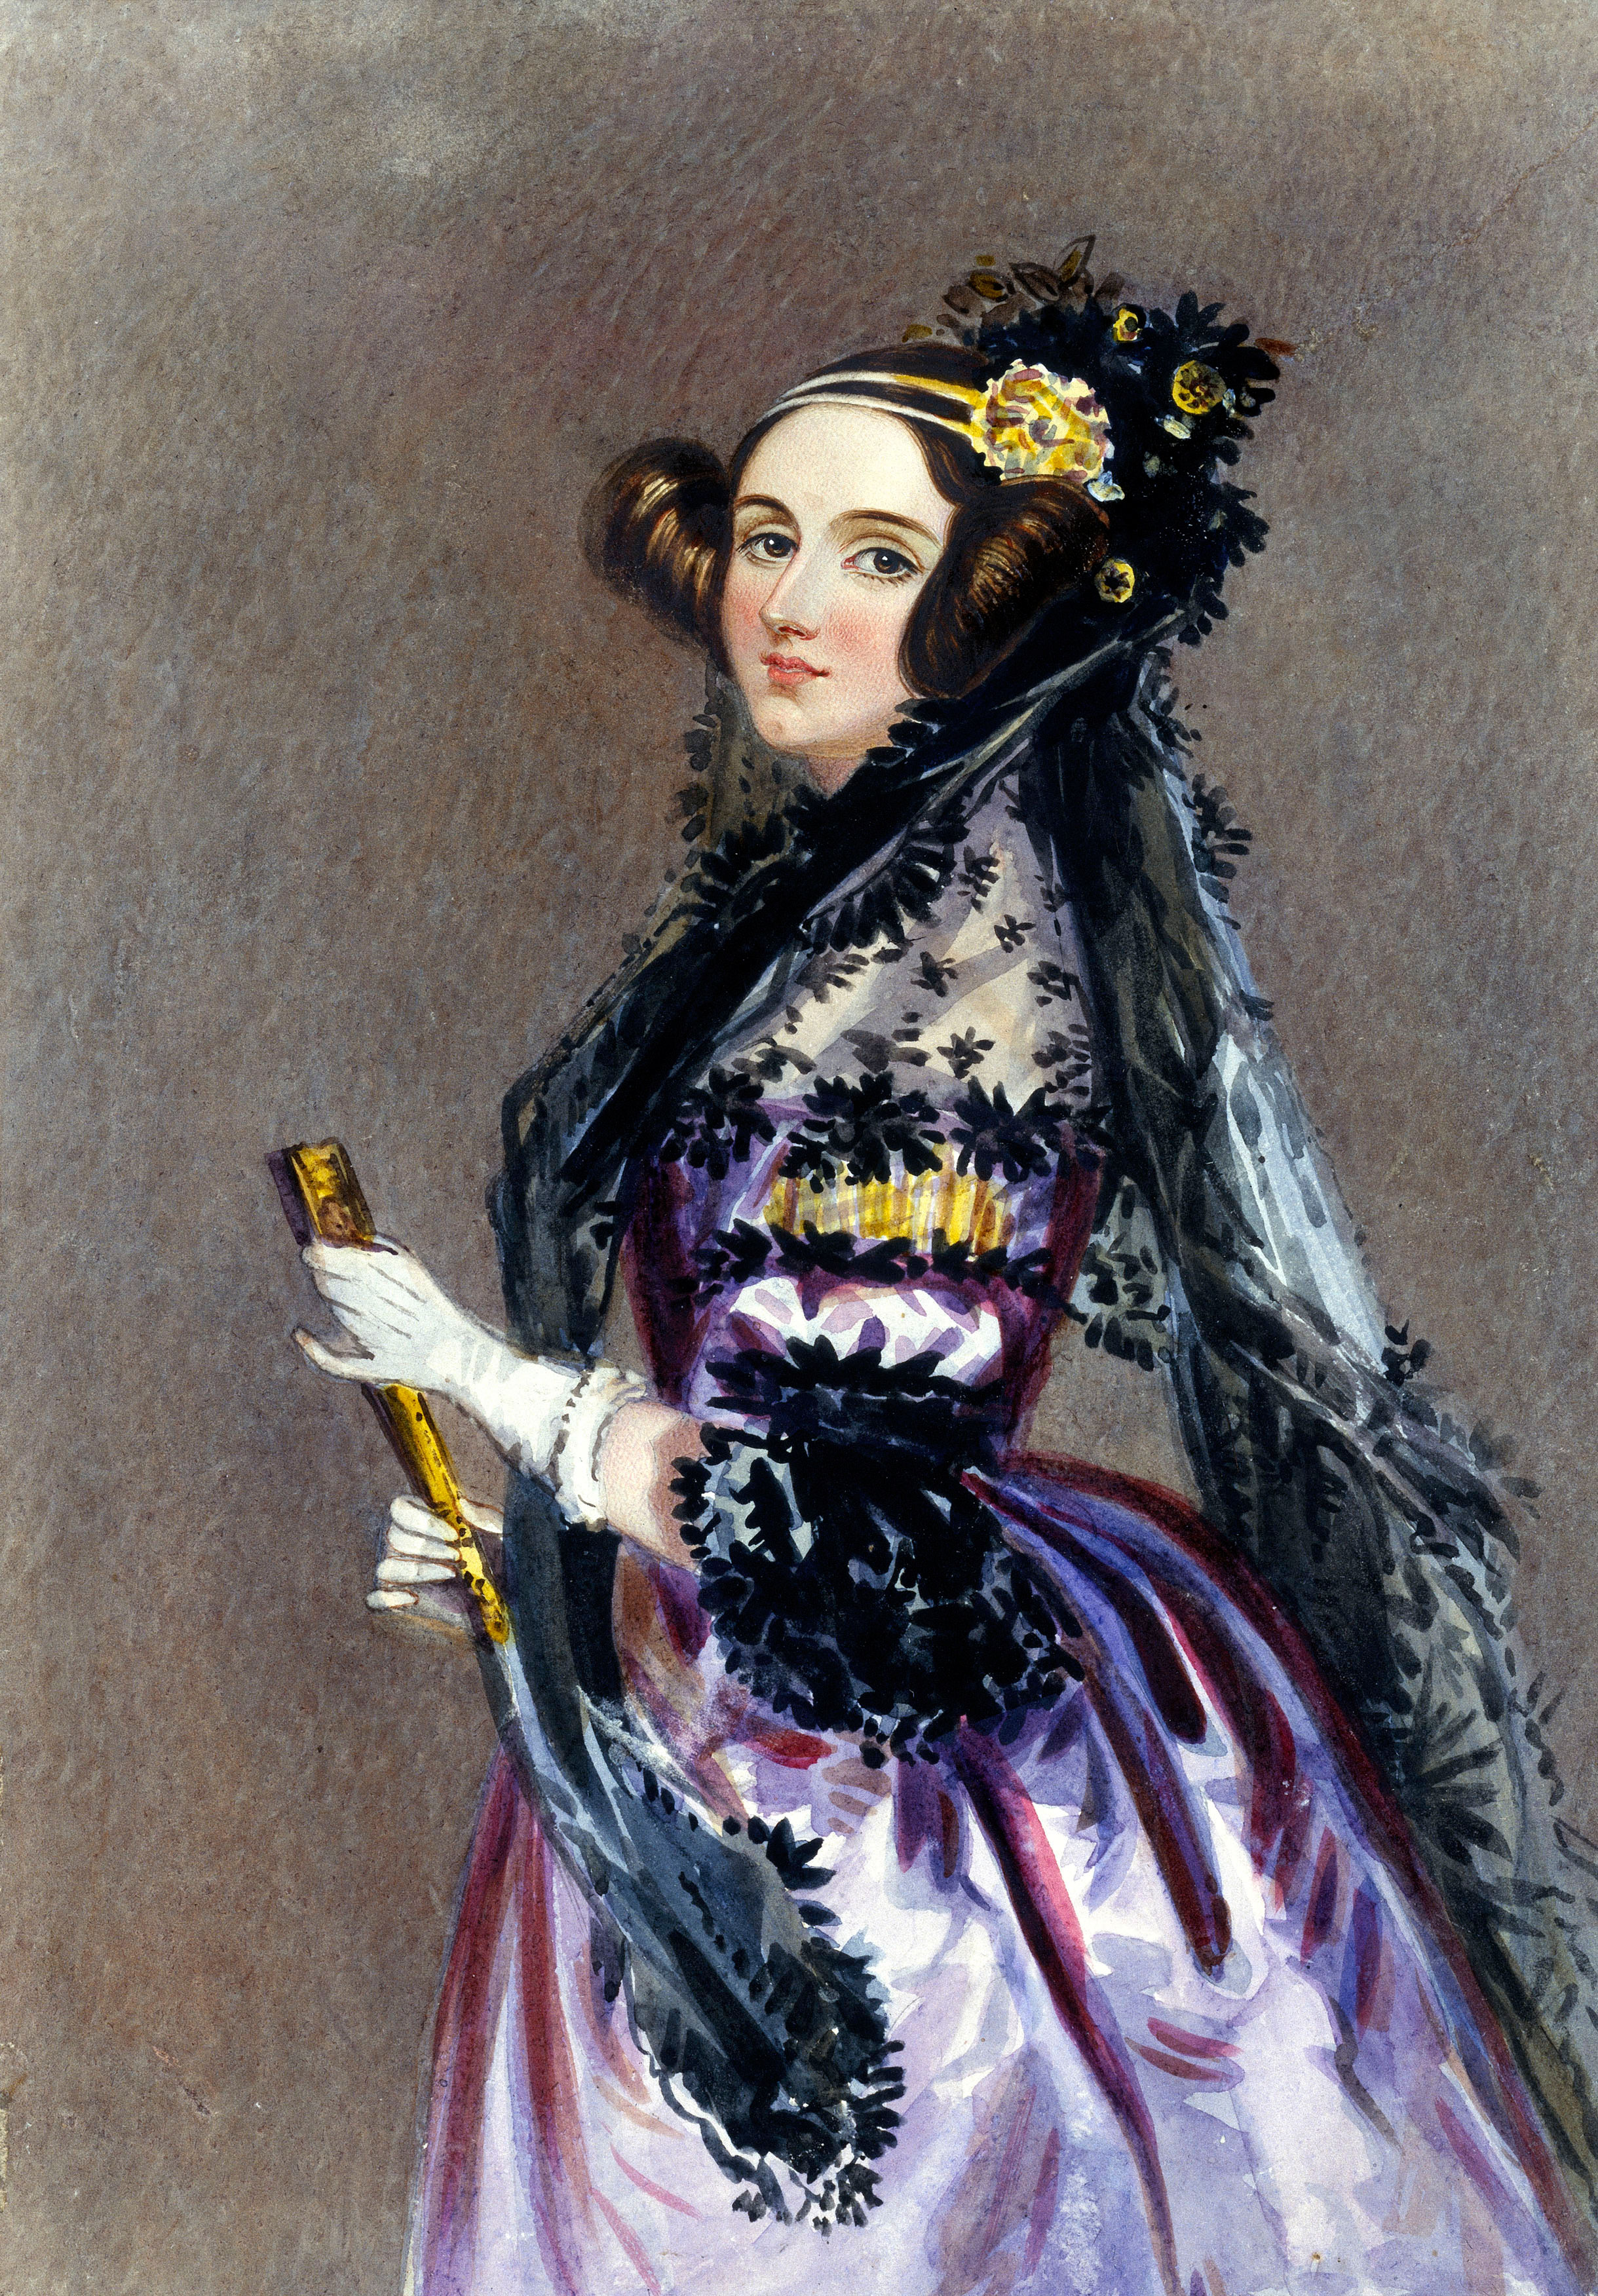
\includegraphics[width = 5 cm]{pic/lovelace} % Include a department/university logo - this will require the graphicx package
\end{center}



\begin{bottompar}
% ---- Professor -----
\begin{flushleft} \large
Dr. \textsc{Catasta} Michele\\
Distributed Information Systems Laboratory (LSIR) \\
\mail{michele.catasta@epfl.ch} \\ 
\end{flushleft}

% ---- date
{\large June 10, 2016}\\[1cm] % Date, change the \today to a set date if you want to be precise

\end{bottompar}
 
\vfill % Fill the rest of the page with whitespace

\end{center}
\end{titlepage}

\clearpage

\tableofcontents 
\newpage

% !TEX root = ../notes.tex

% ================ Introduction ==============
\section*{Course content}

The purpose of the course is to present multiple topics in the data science field such as \emph{Data Wrangling}, \emph{Data Management}, \emph{Data Mining}, \emph{Machine Learning}, \emph{Visualization}, \emph{Statistics} and \emph{Story telling}. The course has not the presumption to go deeply into each argument. It is due to the extent of the subject and the fact that it is evolving really quickly, hence learning in depth a specific tool will not pay off.

\subsection*{Skills to develop}

In this course, you will work, thus develop, the following skills:

\begin{description}
 \item \emph{Data mining/scraping/sampling/cleaning} in order to get an informative, manageable data setlength
 \item \emph{Data storage and management} in order to be able to access data quickly and reliably during subsequent analysis
 \item \emph{Exploratory data analysis} to generate hypotheses and intuition about the data
 \item \emph{Prediction} based on statistical tools such as regression, classification, and clustering
 \item \emph{Communication of results} through visualization, stories and interpretable summaries
\end{description}

\subsection*{Structure of the notes}

The notes of the lectures are put in writing with the aim of summarizing the main topics and concepts illustrated during the classes. To those who are curious, it points to external links that may help you to an in-depth understanding of the field. Each chapter corresponds to a lecture. The hope is that the work could be useful for the current and future students. 


\clearpage

\section{Introduction}

\subsection{What is Data Science?}

When we talk about Data Science, we often use the term Big Data as the enormous amount of data that exists in the world. But Big Data is not only about collecting huge amount of data. It is challenging but not enough. The real value comes from the insights. The {\it internet} companies (Google, Facebook, etc.) 
understood this many years ago.
\\ \\
An accurate definition of Data Analysis is given by Wikipedia:
\begin{framed}
{\it {\bf Analysis of data} is a process of {\bf inspecting}, {\bf cleaning}, {\bf transforming}, and {\bf modeling data} with the goal of {\bf discovering useful information}, suggesting conclusions, and supporting decision-making.
Data analysis has multiple facets and approaches, encompassing diverse techniques under a variety of names, {\bf in different business}, science, and social science {\bf domains}.}
\signed{\href{https://en.wikipedia.org/wiki/Data\_analysis}{Wikipedia - Data Analysis}}
\end{framed}

Therefore, a Data Scientist has to master different kinds of skills such as {\bf Mathematics} , {\bf Statistics}, {\bf Programming} and the {\bf Domain Expertise}. \href{http://videolectures.net/kdd2014\_conway\_social\_science/}{Drew Conway's Venn diagram}, Figure \ref{img:venn}, shows the different combination man can obtain with these three skills.

\begin{figure}[H]
 \centering
 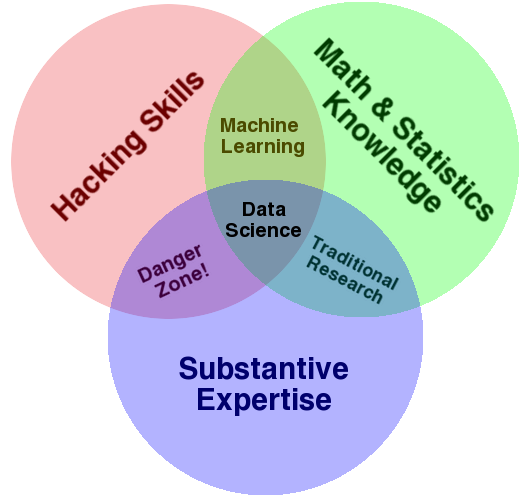
\includegraphics[width=7cm]{./img/01/Data_Science_VD.png}
 \caption{\label{img:venn} Venn Diagram describing the different combination of skills used by a Data Scientist (by Drew Conway)} 
\end{figure}

\begin{figure}[H]
 \centering
 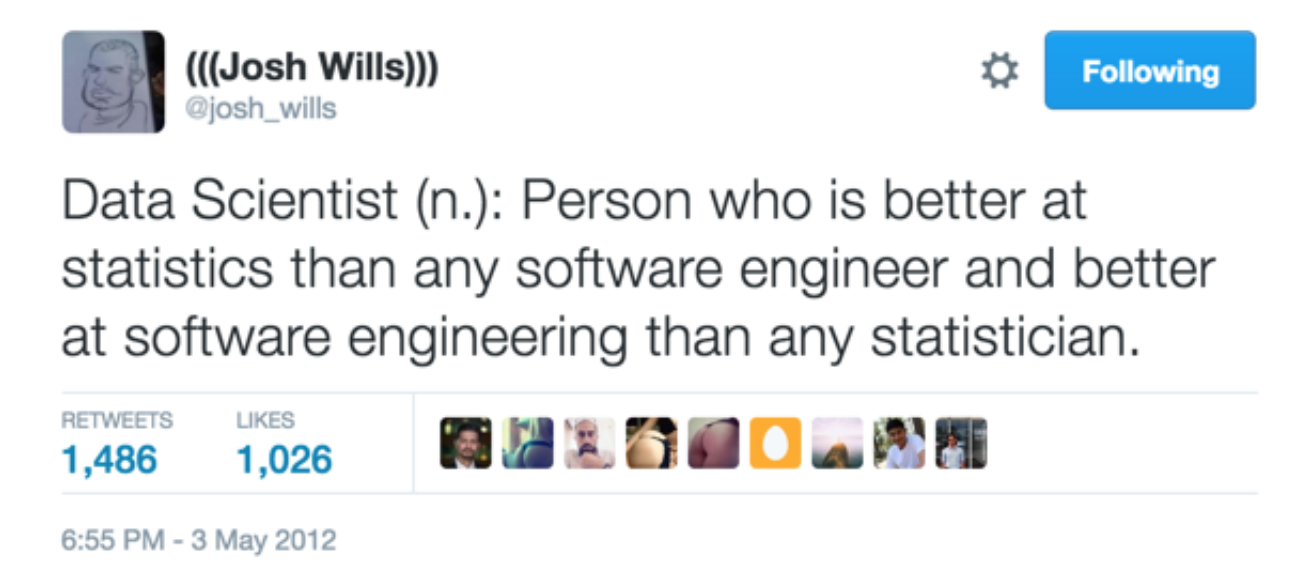
\includegraphics[width=10cm]{./img/01/tweet_wills.png}
 \caption{\label{img:tweet_wills} A tweet from Josh Wills, Data Scientist at Slack.}
\end{figure}

Whether you are interest in knowing what other people think about \emph{Data Science} there are many ongoing \href{https://www.quora.com/What-is-data-science}{discussions}.

{\bf A more practical definition} 

Data Science is about the whole processing pipeline to extract information out of data. As such, a Data Scientist {\bf understands and cares about the whole data pipeline}.

\begin{minipage}{0.5\textwidth}
\begin{figure}[H]
 \centering
 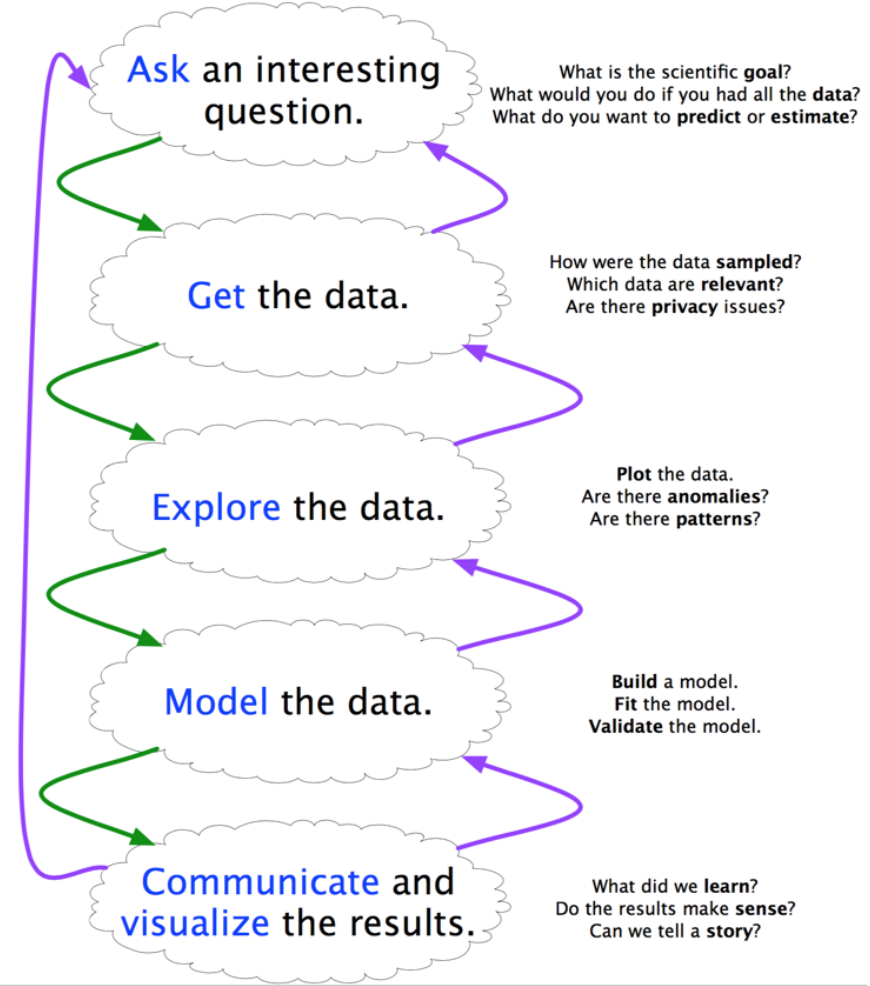
\includegraphics[width=8cm]{./img/01/pipeline.png}
\end{figure}
\end{minipage} \hfill
\begin{minipage}{0.45\textwidth}
A {\bf data pipeline} consists of 3 steps:
\begin{enumerate}
 \item Preparing to run a model: \\
  {\it Gathering, cleaning, integrating, restructuring, transforming, loading, filtering, deleting, combining, merging, verifying, extracting, shaping}
 \item Running the model
 \item Communicating the results
\end{enumerate}
\vspace{0.5cm}
 A ``good'' Data Scientist will always go back and forth between the steps. The diagram on the left shows exactly what can happen. 
\end{minipage}

\clearpage
% !TEX root = ../notes.tex

\section{Basic concepts}
\subsection{A taste of "grammar"}

A data science student is attended to understand the \emph{Grammar of Data Science}. We are going to learn the core data manipulations, so no matter what is the backend is \texttt{SQL, pandas} and \texttt{R}(with \texttt{dplyr}), all share the same\emph{ grammar}. 
For sure having some backgrounds in SQL concepts is a good thing because, as it is very common, people love to make examples with it. Here is a brief refresh of some definitions and concepts that are essential and we need to be aware of.

Let's start with two key concepts that \emph{Structured data} requires:

\begin{itemize}
  \item {\bf Data model}: a collection of concepts for describing data.
  \item {\bf Schema}: a description of a particular collection of data, using a given data model.
\end{itemize}

The most common and ubiquitous approach to manage data is the \emph{Relational model} (\href{https://en.wikipedia.org/wiki/Edgar\_F.\_Codd}{E. F., Ted Codd}). It can handle most of the data, so most of it is "reduced" to this model. To have an idea, a counter example is the facebook-like data which requires {\bf graph model}. 

The \emph{Relational model} is composed by relations. A \emph{relation} is made up two parts:

 \begin{enumerate}
 \item The {\bf Schema} specifies name of relation, plus name and type of each column. \\ For example, \verb+Students(sid: string, name:string, age:integer)+
  \item The {\bf Instance}, {\it i.e.} the data at a given time. \\
  Definitions:
  \begin{itemize}
   \item {\bf Cardinality} is the number of rows (= number of items)
   \item {\bf Degree} or {\bf Arity} is the number of fields ( = number of attributes)
  \end{itemize}
 \end{enumerate}

\subsection*{Database vocabulary}

Here follows a list of basic words and operations that should be kept in mind when we talk about \emph{Databases}.

 \begin{itemize}
  \item A \texttt{JOIN} is a mean to combine tables based on shared attributes (most of the time some \texttt{IDs}). Despite its apparent simplicity beware of the many ways to compute a \texttt{JOIN} and check what is the default \texttt{JOIN} of a language before using it. Every different \texttt{JOIN} operation has implications on the resulting relation. The Figure \ref{join_SQL} summarises these possibilities.
  \item \emph{Aggregation}, \emph{reduction}, and \texttt{groupby} are the actions of reducing data with a common operation (\texttt{sum}, \texttt{count}, \texttt{average}, ...) to summarize them. Remember that you always need to specify the \emph{attribute} you are going to perform the \emph{aggregation} on.
 \end{itemize}
 
 Whether you are not too familiar with \emph{Database} you can go through this \href{https://lagunita.stanford.edu/courses/DB/2014/SelfPaced/about}{course} and look up for what you need.

  
\subsection{Our tools}

During this course and, likely, in your future, to handle data you are going to use a \emph{'magic'} \texttt{Python}'s tool that has a black and white coat, with black fur around its eyes: \texttt{pandas}. 

The basic ingredients of our beloved \texttt{pandas}:

\begin{itemize}
 \item \texttt{Series} are a name, ordered dictionary
\begin{itemize}
 \item keys are indexes
 \item built on \texttt{numpy.ndarray} (so values can be any \texttt{Numpy} data type)
\end{itemize} 
\end{itemize}


\begin{itemize} 
 \item \texttt{DataFrame} is a table with named column
  \begin{itemize}
  \item the columns are series
  \item it is indeed a dictionary with (columnName $\rightarrow$ series)
  \end{itemize}  
\end{itemize}

Learn how to use \href{https://github.com/ADAEPFL/Labs/tree/master/02\%20-\%20Intro\%20to\%20Pandas}{\texttt{pandas}} and discover the beauty of \href{https://github.com/ADAEPFL/Labs/tree/master/01\%20-\%20Intro\%20to\%20Tools}{\texttt{IPython Notebooks}}.

\begin{figure}%---------------FIG--------------
 \centering
 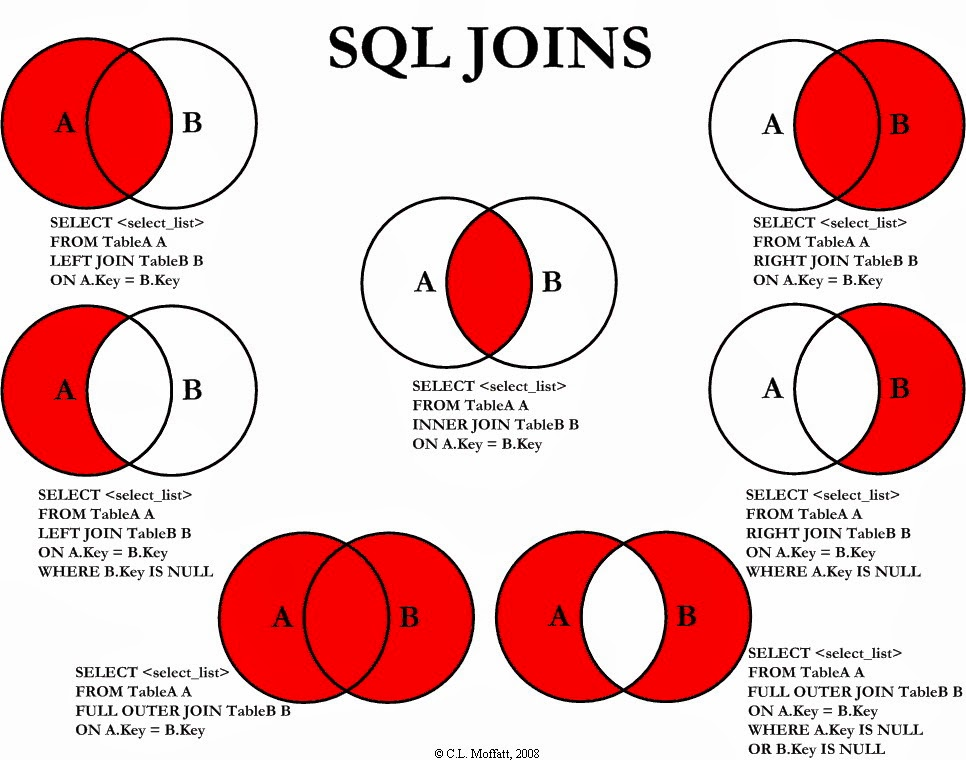
\includegraphics[width=12cm]{./img/02/SQL_joins}
 \caption{\label{join_SQL} Different ways to join two tables and the related SQL command.}
\end{figure}


\subsection{Panda vs SQL}

\texttt{pandas} is built to allow easy and fast \emph{data exploration} and not to be a database manager, as SQL is. Thus there are benefits and drawbacks of using it.


\begin{center} %---------------TAB--------------
\begin{tabular} {| l | l |}
\hline
\bf Pros & \bf Cons \\ \hline
+ Lightweight \& fast & - Tables stored directly in memory \\
+ Great expressiveness (combine SQL + Python) & - No post-load indexing functionality\\
+ Easy plot for data visualization (e.g. Matplotlib) & - No transactions, journalings\\ 
& - Large, complex joins are slower \\ \hline
\end{tabular}
\end{center}

\subsection{OnLine Analytical Processing (OLAP cubes)}

OLAP tools enable users to analyze multidimensional data interactively from multiple perspectives. Conceptually, it is like an n-dimensional spreadsheet (a cube) on which we can apply various operations to take decisions.

OLAP cubes are another way to see data tables and are constructed based on them, as shows Figure \ref{OLAP_cubes}.

\begin{figure}[H]%---------------FIG--------------
 \centering
 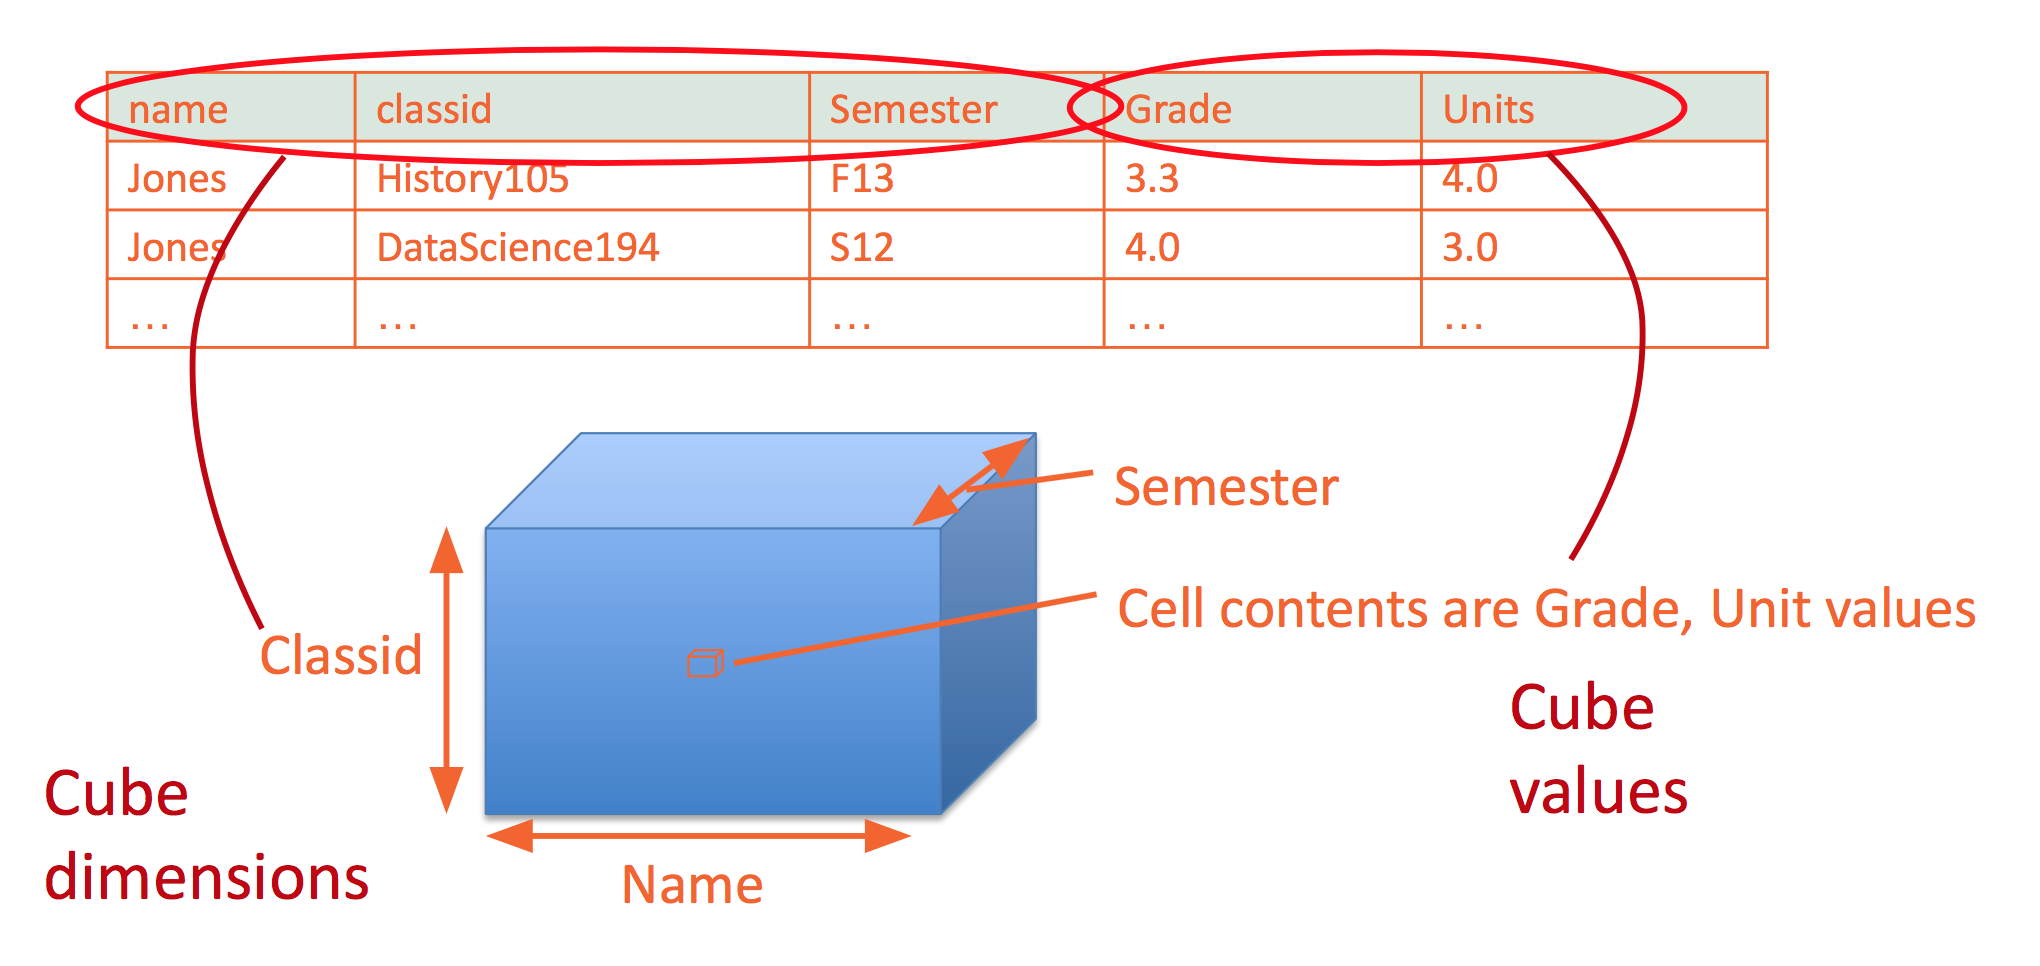
\includegraphics[width=12cm]{./img/02/OLAP_cube}
 \caption{\label{OLAP_cubes} Construction of an OLAP cube from a table.}
\end{figure}

Operations on OLAP cubes are the following and are illustrated on Figure \ref{OLAP_operations}
\begin{itemize}
	\item \emph{Slicing} fixes one or more variable
	\item \emph{Dicing} selects a range of one or more variable
	\item \emph{Drilling up/down} change levels of a hierarchically indexed variable, i.e. "zoom" on a variable and see the subcategories it contains.
	\item \emph{Pivoting} change the point of view of the cube. Swap an aggregated variable and a detailed one.
\end{itemize}

\begin{figure} [h] %----------- SubGraph ---------------------
\centerline{
\subfigure[Slincing\label{olap_slicing}] {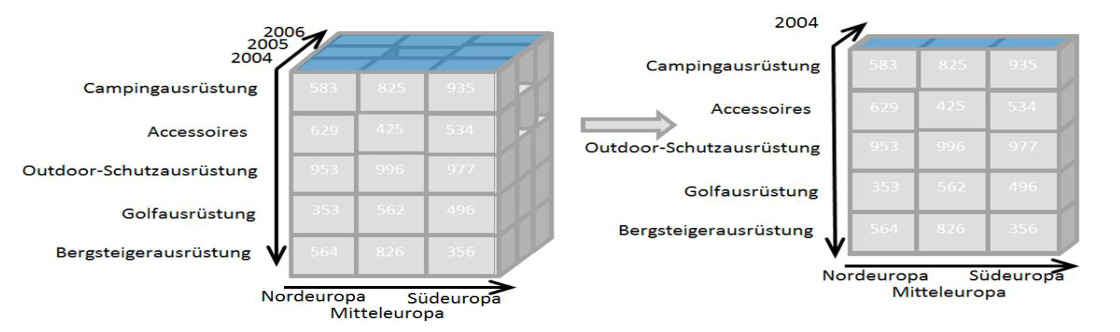
\includegraphics[width=7cm]{img/02/Slicing} }
\subfigure[Dicing\label{olap_dicing}] {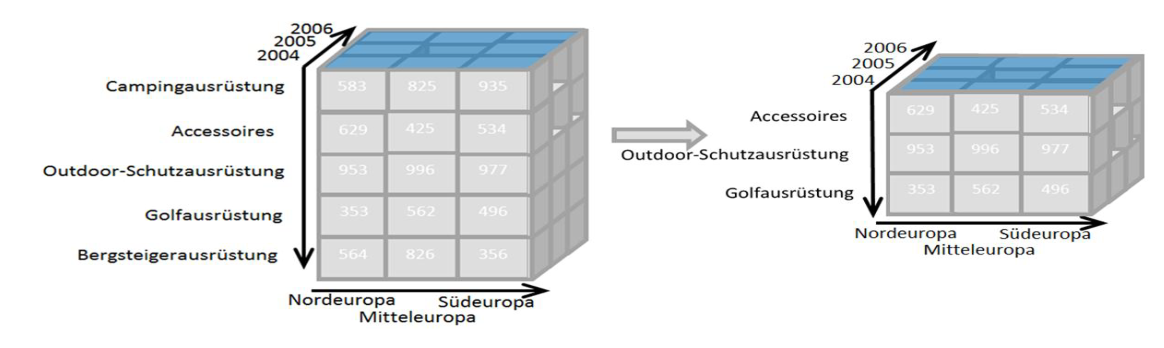
\includegraphics[width=7cm]{img/02/Dicing} } 
}
\centerline{
\subfigure[Driling up/down\label{olap_driling}] {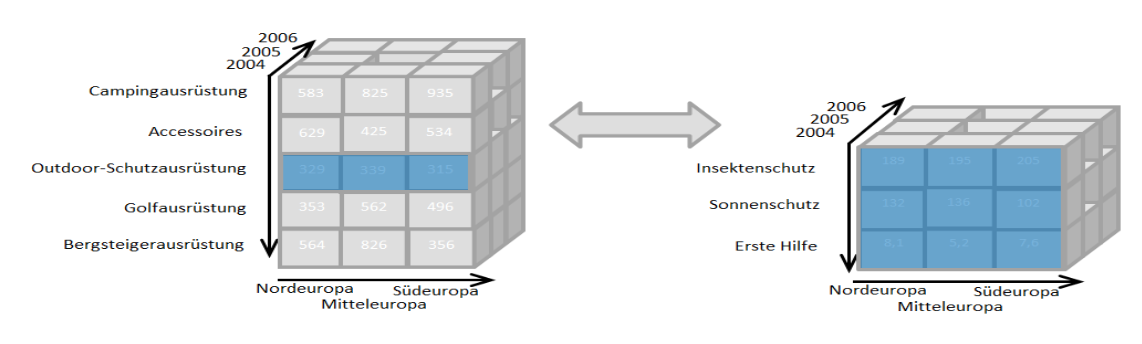
\includegraphics[width=7cm]{img/02/Drilling_up_down} }
\subfigure[Pivoting\label{olap_pivoting}] {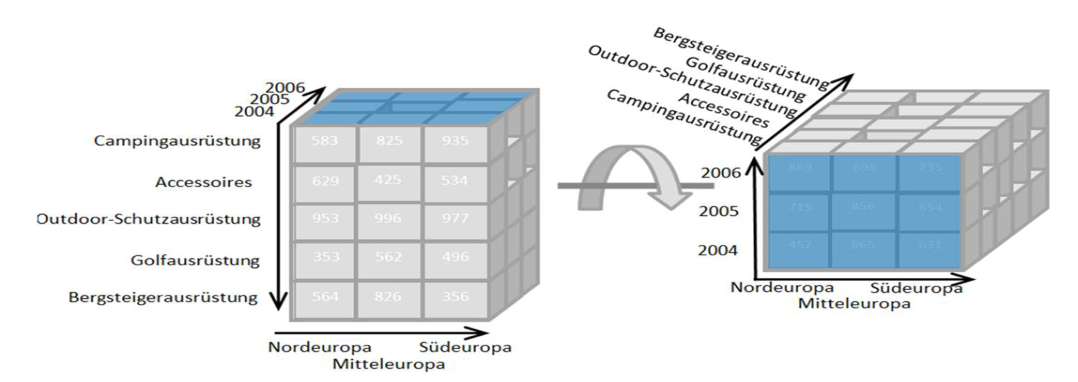
\includegraphics[width=7cm]{img/02/Pivoting} } 
}
\caption{\label{OLAP_operations} Operations on OLAP cubes} 
\end{figure}

\begin{center} %---------------TAB--------------
\begin{tabular} {| l | l |}
\hline
\bf Pros & \bf Cons \\ \hline
& \\
\parbox[t][][t]{7cm}{+ The main advantage of OLAP cubes is that they are \textbf{conceptually simpler} to understand by a non-scientist person, e.g. a business man who has to take day-to-day decisions based on company's data. Aggregations are limited but cover the main common cases that we can encounter.
}&
\parbox[t][][t]{7cm}{- Because of the "on-line" behaviour of this approach, all types of aggregation must be pre-calculated among all combinations of axes which is very \textbf{expensive in memory and in time} (when updating the data)}\\
& \\
\hline
\end{tabular}
\end{center}

\clearpage

\clearpage
% !TEX root = ../notes.tex

% ================ Data Wrangling ==============
\section{Data Wrangling}

\begin{figure}[H]%---------------FIG--------------
 \centering
 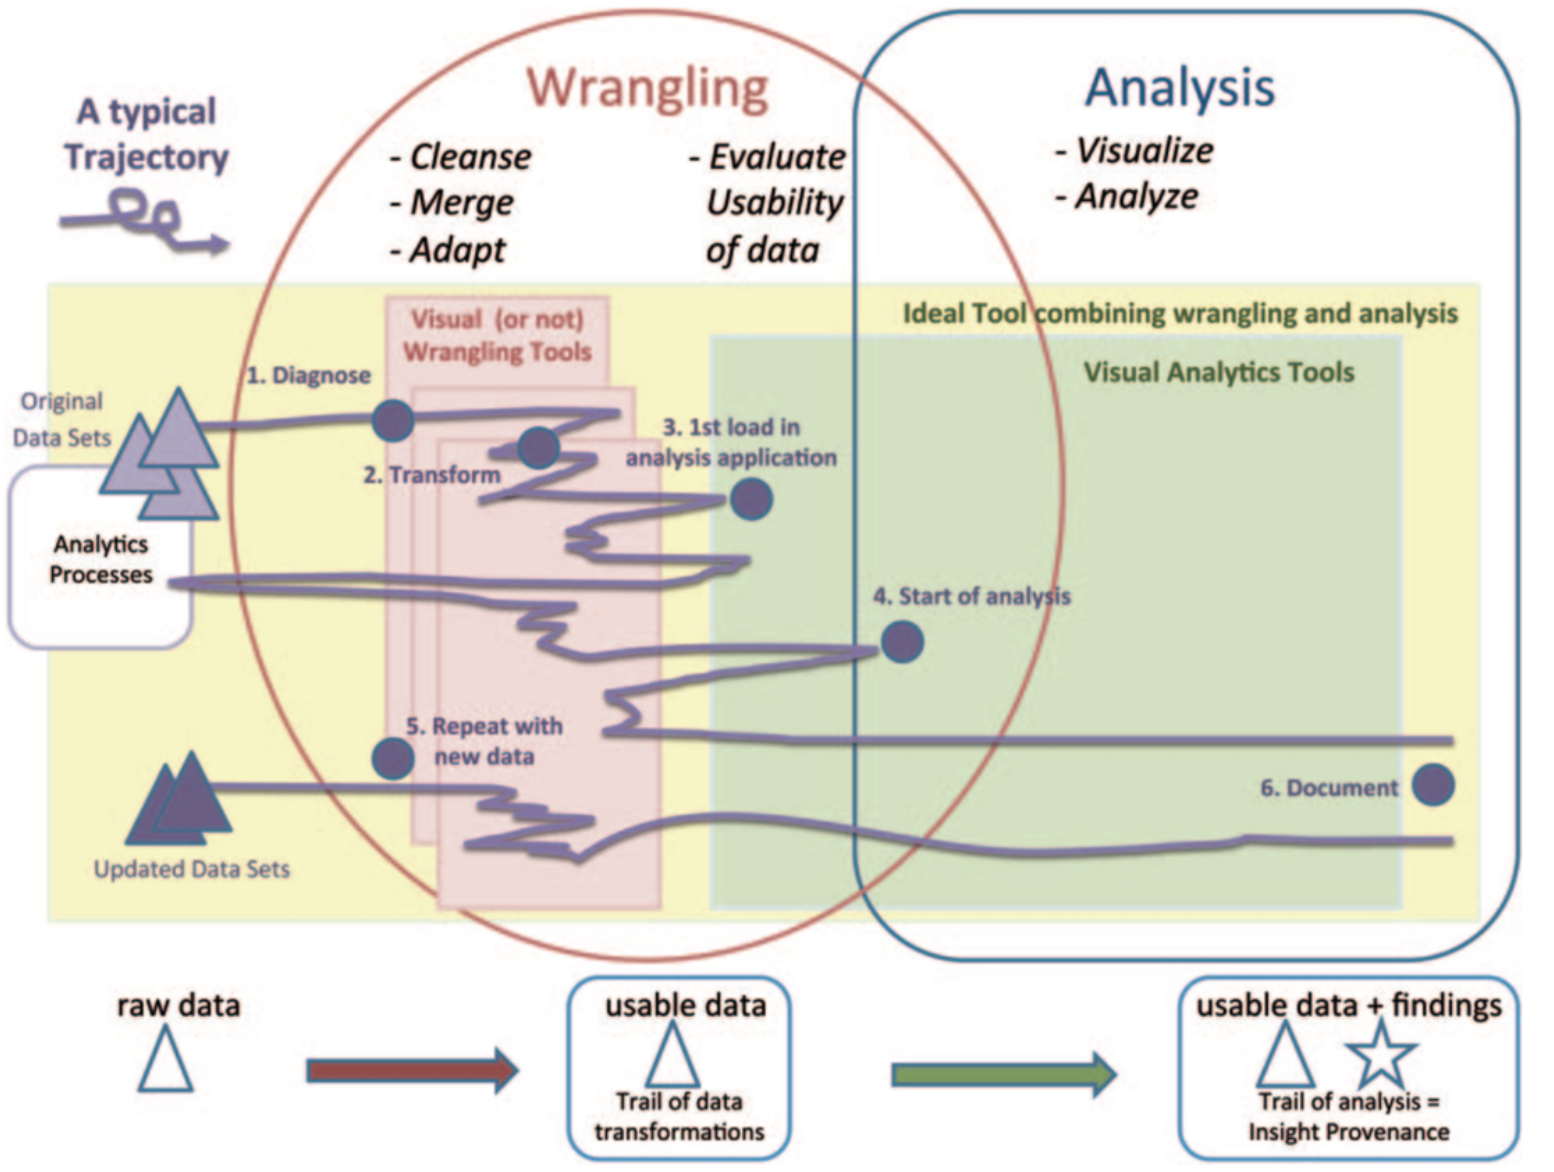
\includegraphics[width=12cm]{./img/03/path_data_wrangling}
 \caption{\label{path_data_wrangling}Things do not always happen as expected...}
\end{figure}

Before any analysis, data need to be transformed from "dirty" to clean and processable data.

Data come from different sources, sometime collected through different methods over time, with different conventions. Generally, it leads to unwanted anomalies and duplicates. \emph{Data wrangling} goal is to \textbf{extract and standardize these raw data}. The best way to do it is to \textbf{combine} automation with visualizations in order to proceed with the cleaning. 

Here is a \emph{non-exhaustive} list of where data problems can come from: 
\begin{itemize}
  \item \emph{Missing data}
  \item \emph{Incorrect data}
  \item \emph{Inconsistent representations of the same data}
  \item \emph{Non-standardized data (centimeter or inches? Fahrenheit or Celsuis ?)}
  \item \emph{Duplicated data}
\end{itemize}

About 75\% of theses problems will need \textbf{human intervention} to be corrected (by the data-scientist or by crowdsourcing). Some examples of good data leading to horrible conclusion can be found here: \href{https://www.linkedin.com/pulse/dirty-data-horror-stories-when-michael}{Dirty Data Horror Stories}.

Even if it seems really dirty, \textbf{beware not to over-sanitize the data!} Applying what we can call "defensive programming" is not a good idea because we risk losing any interesting data, keeping only the ones that fit perfectly in our model.

Anyway, a good \emph{Data wrangling} procedure brings about improvements in the efficiency and scale of data importing.

\subsection{Diagnosis of the data}

One of the most important aspects of Data Wrangling is to {\bf understand} the data and to {\bf find} possible problems. In order to "diagnose'' the data, two tools can be used:
\begin{itemize}
 \item {\emph Visualization} (A {\it thoughtful} visualization will always help)
 \item {\emph Basic Statistics} 
\end{itemize}

Look out, outliers and missing data can be often identify using a plot. Visualization becomes increasingly difficult when  \href{http://fellinlovewithdata.com/guides/how-do-you-visualize-too-much-data}{data gets larger}.

Matrix visualizations of the facebook graph is shown in Figure \ref{pic:fb}. The Relational visualization, Figure \ref{pic:fb1}, does not show any particular problem in the data. But the Time dependant visualization, Figure \ref{pic:fb2}, shows that the Facebook API reached its limit while collecting data.

\begin{figure} [h] %----------- SubGraph ---------------------
\centerline{
\subfigure[Relational visualization \label{pic:fb1}] {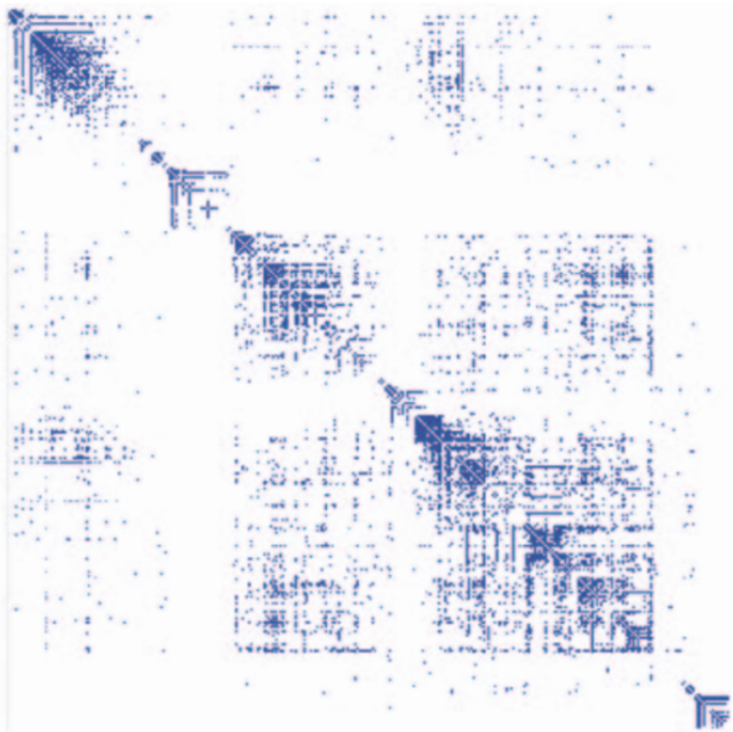
\includegraphics[width=7cm]{img/03/fb1} }
\subfigure[Time dependant visualization\label{pic:fb2}] {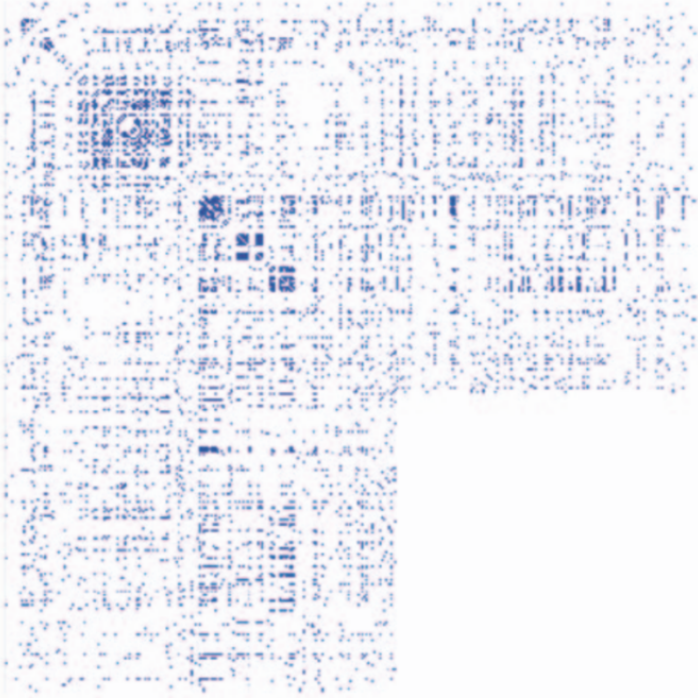
\includegraphics[width=7cm]{img/03/fb2} } 
}
\caption{\label{pic:fb} Matrix visualization of the facebook graph.} 
\end{figure}


\subsection{Dealing with missing values}

Values can often miss from the data we have, because of various events (war, fire, ...). We must detect and correct these values with different methods according to the domain we are working in.

Whatever the method used, it's good to keep track of these changes to know which are original data and which are modified ones.

\begin{itemize}
  \item Set values to zero Figure \ref{miss_val}(a)
  \item Interpolate based on existing data Figure \ref{miss_val}(b)
  \item Omit missing data Figure \ref{miss_val}(c)
  \item Interpolation with tracks kept Figure \ref{miss_val}(d)
\end{itemize}

\begin{figure}[H]%---------------FIG--------------
 \centering
 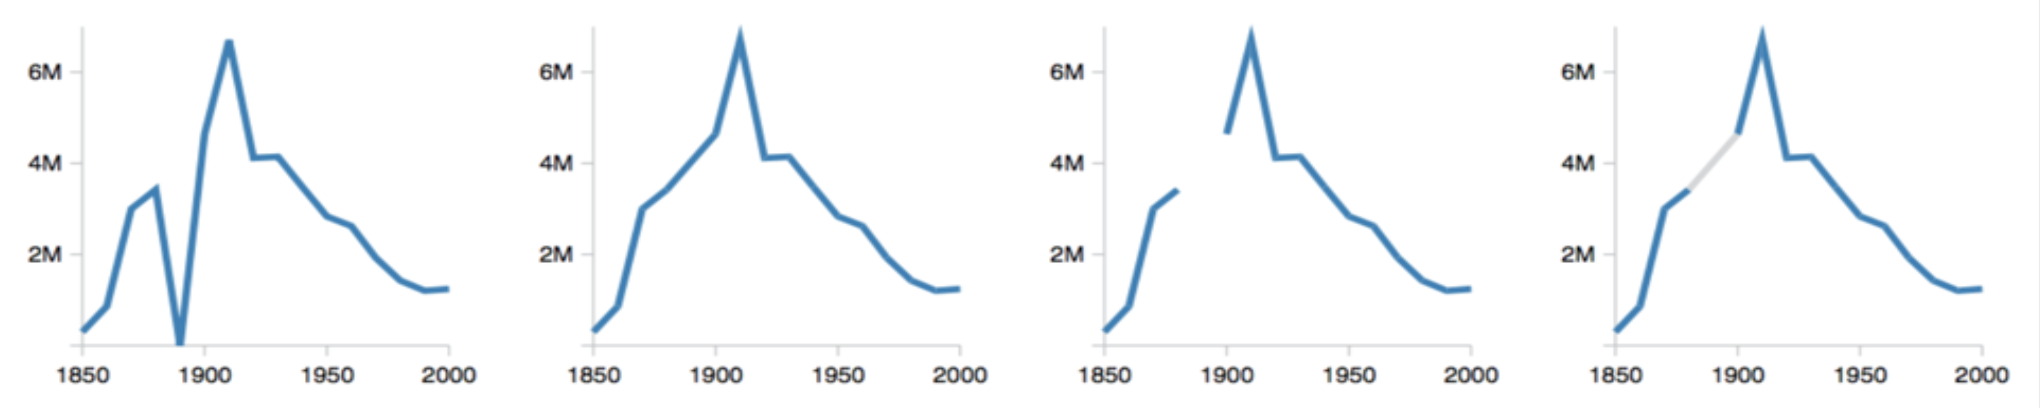
\includegraphics[width=15cm]{./img/03/missing_values}
 \caption{\label{miss_val}To deal with missing values.}
\end{figure}

\subsection{General procedure}

Once the data are well wrangled and before trying to analyze them, we must take care of two more steps:

\begin{enumerate}
  \item \textbf{Deal with uncertain data} (can arise from measurement errors, wrong sampling strategies, etc.)
  \item \textbf{Parse/transform data} (with aggregation and reduction techniques) to obtain meaningful records
\end{enumerate}
 
As we say in the Introduction, \emph{Data Science} is a mixture of different fields. It often leads to the necessity of working in team where different people have different skills. Working in a team means sharing code, documentation and data. Hence, taking care of them is essential.

\clearpage


 
\clearpage
% !TEX root = ../notes.tex

% ================ Data Variety ==============
\section{Data Variety}

The \href{http://blog.sqlauthority.com/2013/10/02/big-data-what-is-big-data-3-vs-of-big-data-volume-velocity-and-variety-day-2-of-21/}{``3 Vs'' of Big Data}: {\it Volume}, {\it Velocity} and {\it Variety}. In this course, we don't address the {\it Volume} and {\it Velocity} parts (A course on Database does). Since there is a lot of variety in the data, we need to prepare the data. This flow is called {\bf ETL}:
\begin{itemize}
 \item {\bf Extract} from the {\it source(s)}.
 \item {\bf Transform} data at the source, sink, or in a {\it staging area}.
 \item {\bf Load} data into the {\it sink}.  
\end{itemize}
This variety of the data comes, in a first place, from the many different sources from which we extract them: {\it files, databases, logs, ... } Each of these sources uses (or not!) its proper convention and can contain structured (DB), semi-structured (logs) or unstructured (web page) data. 

\subsection{Role of Schema}
The {\bf Schema}, which specifies the {\it structure} and {\it types} of data repository, is changing. Traditional databases are {\bf schema-on-write}, {\it i.e.} you cannot load data into a table without a schema. But new data stores (NoSQL for example) are {\bf schema-on-read} or {\bf schemaless}. 

\begin{itemize}
	\item {\bf Schema-on-write} is typically SQL, where we must create a table before inserting data in our system. Data must scale the defined schema and this is both the strength and weakness of the system. Strength because the data is perfectly oriented and respect the constraints we establish. Weakness because schemas are always subjective in some ways and data (which are perfectly correct) may not fit with it. 
	\item {\bf Schema-on-read} is for instance XML, where you create the schema according to the data you read.
	\item Youtube and Google Cache where the first {\bf schemaless} data system. Without schema, everything is simply stored as a string and we need a parser to return a typed data.
\end{itemize}

\subsection{Examples of data}

\subsubsection{\href{https://en.wikipedia.org/wiki/XML}{XML} and \href{https://en.wikipedia.org/wiki/Document\_Object\_Model}{DOM}}

The XML data are used mostly with HTML and specifies the data structure. An XML schema can be applied to interpret the XML data and specifies the {\bf data types}. Figure \ref{fig:xml_data} shows the XML data and Figure \ref{fig:xml_schema} shows the schema used to parse and type the data.

\begin{figure}[H]%---------------FIG--------------
 \centering
  \begin{lstlisting}[language=XML]
    <location>
      <latitude>37.78333</latitude>
      <longitude>122.4167</longitude>
    </location>
  \end{lstlisting}
 \caption{\label{fig:xml_data} XML data defined by the schema in Figure \ref{fig:xml_schema}.}
\end{figure}

\begin{figure}[H]%---------------FIG--------------
 \centering
  \begin{lstlisting}[language=XML]
    <xsd:schema xmlns:xsd="http://www.w3.org/2001/XMLSchema" elementFormDefault="unqualified">
    <xsd:complexType name="location">
      <xsd:sequence>
	<xsd:element name="latitude" type="xsd:decimal"/>
	<xsd:element name="longitude" type="xsd:decimal"/>
      </xsd:sequence>
    </xsd:complexType name="location">
  \end{lstlisting}
 \caption{\label{fig:xml_schema} XML schema for the XML data in Figure \ref{fig:xml_data}.}
\end{figure}

The XML is a text format that encodes {\bf DOM} (Document-Object Models). It's a data structure often used by Web pages. The DOM is tree-structured. An example of a DOM is given in Figure \ref{pic:dom}.

\begin{figure}[H]%---------------FIG--------------
 \centering
 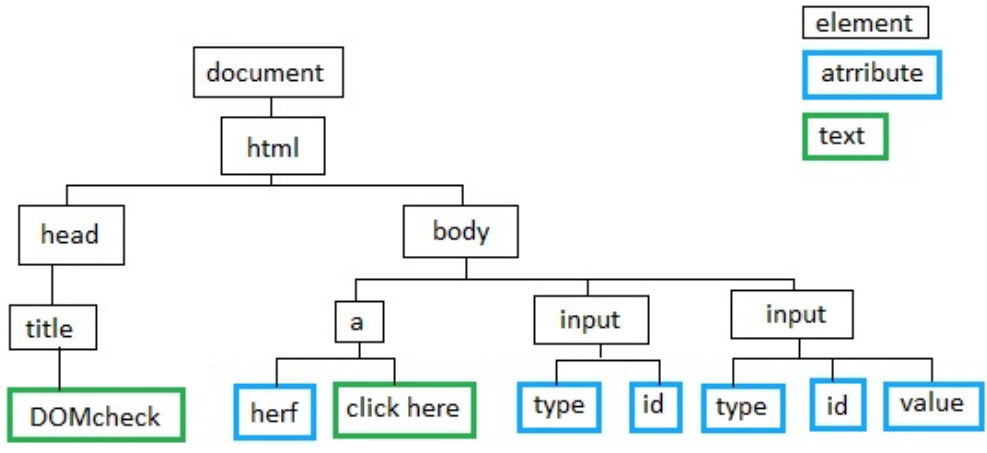
\includegraphics[width=15cm]{./img/04/dom}
 \caption{\label{pic:dom} Example of a DOM tree for an HTML Web page. See example on \href{http://www.w3schools.com/xml/dom_intro.asp}{W3Schools}.}
\end{figure}

THe XML schema allows a database to interpret the data when running queries. It can do arithmetic or range queries on numerical values, for example.

\subsubsection{\href{https://en.wikipedia.org/wiki/JSON}{JSON}}

{\bf JSON} stands for Javascript Object Notation. It's a schemaless data (schema support was added later). An example of JSON data is shown in Figure \ref{pic:json}

\begin{figure}[t]%---------------FIG--------------
  \begin{lstlisting}[language=json]
  {
    "firstName": "John",
    "lastName": "smith",
    "age": 25,
    "address": {
      "streetAddress": "21 2nd Street",
      "city": "New York",
      "state": "NY",
      "postalCode": "10021-3100"
    },
    "phoneNumbers": [
      {
	"type": "home",
	"number": "212 555-1234"
      },
      {
	"type": "office",
	"number": "646 555-4567"
      }
    ],
    "children": [],
    "spouse": null
  }
  \end{lstlisting}
 \caption{\label{pic:json} Example of a JSON data.}
\end{figure}



JSON is typically used to represent {\bf hierarchical data structures} directly in the target language (Javascript or Java at the beginning). The transformation on the data is procedural in the target languages. It is often easier for some tasks, but it can be painful for some of them: for example schema changes.

\subsubsection{Tabular data}

A Tabular Data is simply data put into a table such as CSV (Comma Separated Value) or TSV (Tab Separated Value). Definition of a table:
\begin{itemize}
 \item A {\bf table} is a collection of {\bf rows} and {\bf columns}.
 \item Each row has an {\bf index}.
 \item Each column has a {\bf name}.
 \item A {\bf cell} is specified by an (index, name) pair.
 \item A cell may or may not have a {\bf value}.
\end{itemize}

It's a very simple yet powerful data type. For example, the sensors usually output data in the form of time series, transformed into a tabular format. However, a system dealing with sensor data should:
\begin{itemize}
 \item support both long-term ({\bf trend}) and short-term ({\bf real-time}) queries
 \item have {\bf low latency} but also efficient. It should use {\bf real-time indexing} for longer-term queries.
 \item support triggers ({\bf alerts}) for a variety of conditions.
\end{itemize}
Therefore, the {\bf complexity of a data format} does not determine the {\bf complexity of the system required to properly handle it}.

\subsubsection{Log files}

The log files are simple text files giving information about the process. The daemons, such as \verb+httpd+, \verb+mysqld+ or \verb+syslogd+, usually create logs. {\bf \verb+syslog+} was developed by Eric Allman. It's a way for devices to send event messages to a server that will log all the events. Splunk is a company that built a successful business model around the syslog events.

\subsubsection{Binary formats}

They are often the key to performance because we {\bf avoid expensive parsing}. The modern formats even support nested structures, various levels of schema enforcement, {\bf compression}, etc. Some examples: \href{https://developers.google.com/protocol-buffers/docs/overview}{Protocol Buffers (Google)}, \href{https://avro.apache.org/docs/current/}{Avro (Apache)}, \href{https://parquet.apache.org/documentation/latest/}{Parquet (Apache)}, etc.

\subsection{Processing the data (JSON and XML)}

In order to process XML, we can use the DOM. It can also be used to process JSON data. The DOM is very easy to work with: all the data are directly accessible by links. The problem is that we {\bf might not care about most of the data} and if the data are big, they {\bf might not fit into the RAM}. In order to deal with these two problems, we can use a {\bf SAX} parser which is an event-driven parser. It will find all the {\bf open-close-tag events} in an XML document and will {bf do callbacks to user code}.

\begin{itemize}
 \item[{\bf +}] User code can respond to only a subset of events corresponding to the tag it is interested in.
 \item[{\bf +}] User code can correctly compute aggregates from the data rather than create a record for each tag.
 \item[{\bf +}] User code can implement flexible error recovery strategies for ill-formed XML.
 \item[{\bf --}] User code must implement a state machine to keep track of ``where it is'' in the DOM tree.
\end{itemize}

For JSON, most parsers construct the ``DOM'' directly. But there are a few SAX-style parsers: Jackson, JSON-simple, etc. Sometimes {\bf SAX-style is the way to handle ill-formed datasets}, an endless array of objects, for example.

\subsection{HTML and Web Services}

\subsubsection{HTML}

Internet contains an ``enormous'' amount of data. Some crawlers such as Common Crawl datasets contains about 1.82 billion web pages (for 145 TB). We can use different tools to crawl data from the web. Examples for Python: Beautiful Soup, Requests, Scrapy, etc. 
\\\\
Most of the time, the Web pages are considered as unstructured data. But you can find some semi-structured data, {\it e.g.} Google WebTables. Some big ``internet'' companies (Google, Yahoo, Yandex and Microsoft) are sponsoring a project called \href{http://schema.org/}{schema.org} to create structured or semi-structured Web pages. A core vocabulary for the type of fields is given. schema.org is more and more used. It's also used by knowledge bases such as Google Knowledge Graph. \href{https://www.wikidata.org/wiki/Wikidata:Main\_Page}{WikiData} is a community project to create an open database of structured data taken from Wikipedia.

\subsubsection{Web Services}

Screen-scraping the content of a large website was possible before, but become more and more difficult nowadays. This is mainly due to the content "hidden" behind a form or an authentification. Take for example facebook without account, or the IS-academia course page if you do not select a semester. Therefore big companies are providing Web Service APIs\footnote{Application Program Interface: Set of subroutine definitions, protocols, and tools for building software and applications. In this particular case, the APIs are used to retrieve the data from the Web page, {\it e.g.} Facebook API to retrieve the contacts.} to retrieve data from their website. There are two kinds of Web Services:
\begin{itemize}
 \item The old way: XML-based RPC-style messages: SOAP
 \item The new way: REST-style stateless interactions, URLs encode state
\end{itemize}

\paragraph{RPC}

The SOAP RPC \footnote{SOAP = Simple Object Access Protocol, RPC = Remote Procedure Call} messages typically encode arguments that are presented to the calling program as parameters and return values. HTTP POST/GET are used to communicate.
\begin{figure}[H]%---------------FIG--------------
 \centering
 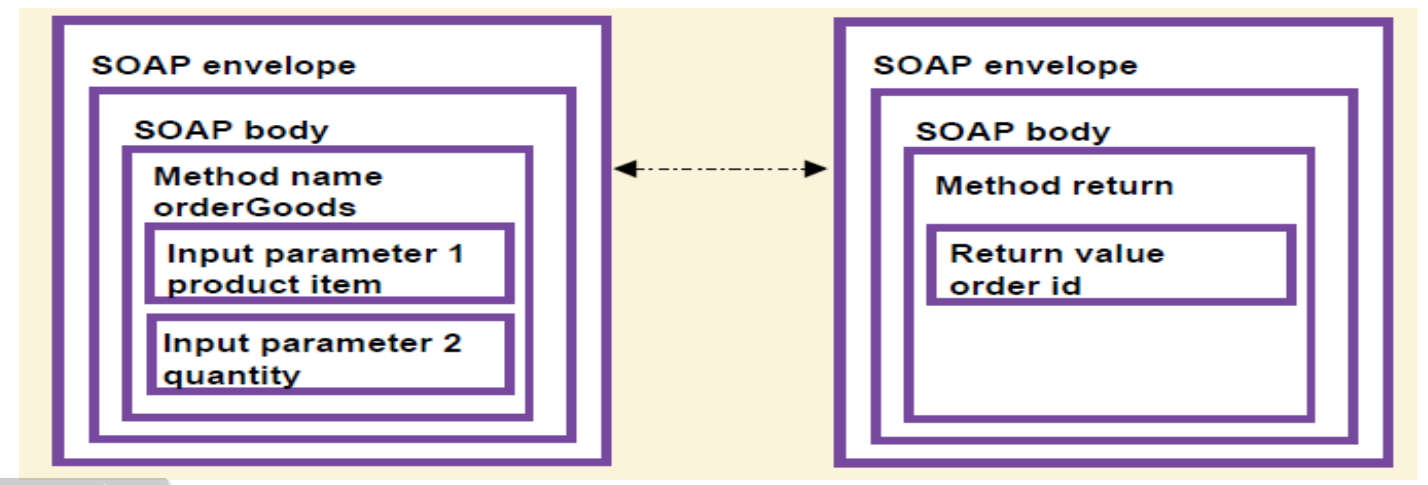
\includegraphics[width=13cm]{./img/04/soap-rpc}
 \caption{\label{pic:soap-rpc} Example of a SOAP RPC exchange.}
\end{figure}
This kind of procedure (same for XML-RPC) requires a request-response cycle. This often leads to longer ``conversations''. The RPC-style is being quickly superseded by newer and more user-friendly technologies.\\\\
In {\bf RPC systems}, the design emphasis is on {\bf verbs}. It uses functions such as {\it getUser()}, {\it addUser()}, etc.


\paragraph{REST}

REST\footnote{REpresentation State Transfer} is a {\bf stateless} client/server protocol. The principles are:
\begin{enumerate}
 \item Each message in the protocol contains all the information needed by the receiver to understand and/or process it. This constraint attempts to {\it ``keep things simple''} and avoids needless complexity.
 \item Set of Uniquely Addressable Resources
 \begin{itemize}
  \item {\it ``Everything is a Resource''} in a RESTful system
  \item Requires universal syntax for resource identification, {\it e.g.} URI.
 \end{itemize}
 \item Set of Well-Defined Operations that can be applied to all resources
 \begin{itemize}
  \item In the context of HTTP (REST APIs), the primary methods are: \\
  {\bf POST}, {\bf GET}, {\bf PUT}, and {\bf DELETE} \\
  These are similar (but not exactly) to the database notion of CRUD (Create, Read, Update, and Delete)
 \end{itemize}
 \item The use of Hypermedia both for Application Information and State Transitions
 \begin{itemize}
  \item Resources are typically stored in a structured data format that supports hypermedia links, such as XHTML or JSON.
 \end{itemize}
\end{enumerate}
In {\bf REST systems}, the design emphasis is on {\bf nouns}. It uses the HTTP Protocols (POST, GET, PUT, and DELETE) a {\it User}, a {\it Location}, etc. 

\clearpage





\clearpage
% !TEX root = ../notes.tex

% ================ Statistics ==============
\section{Statistics on the Data}

When we explore and analyze data, it would be great if we only had to look at some statistics numbers and make automatically a conclusion about them. Sadly, it's not the case. At all.
% ================  Famous mistakes ==============
\subsection{Examples of famous mistakes due to statistics}

%=================== Anscombe's quartet ===================
\subsubsection{Anscombe's quartet: Sensivity of outliers \& Robust statistics}

The FIG \ref{pic:anscombe} show four different data distribution that present, despite all of that, the same means on $x$ and $y$, the same variance on $x$ and $y$, and, thus, the same linear regression function. This is due to the statistics used to define them. 

\begin{itemize}
    \item Min, Max, Mean, Standard Deviation (Std) and Range are sensitive to outliers and then are \textbf{not robust statistics}.
    \item Median, quartils, (and others) are not sensitive and then are said to be \textbf{robust statistics}. 
\end{itemize}



\begin{figure}[h]%---------------FIG--------------
 \centering
 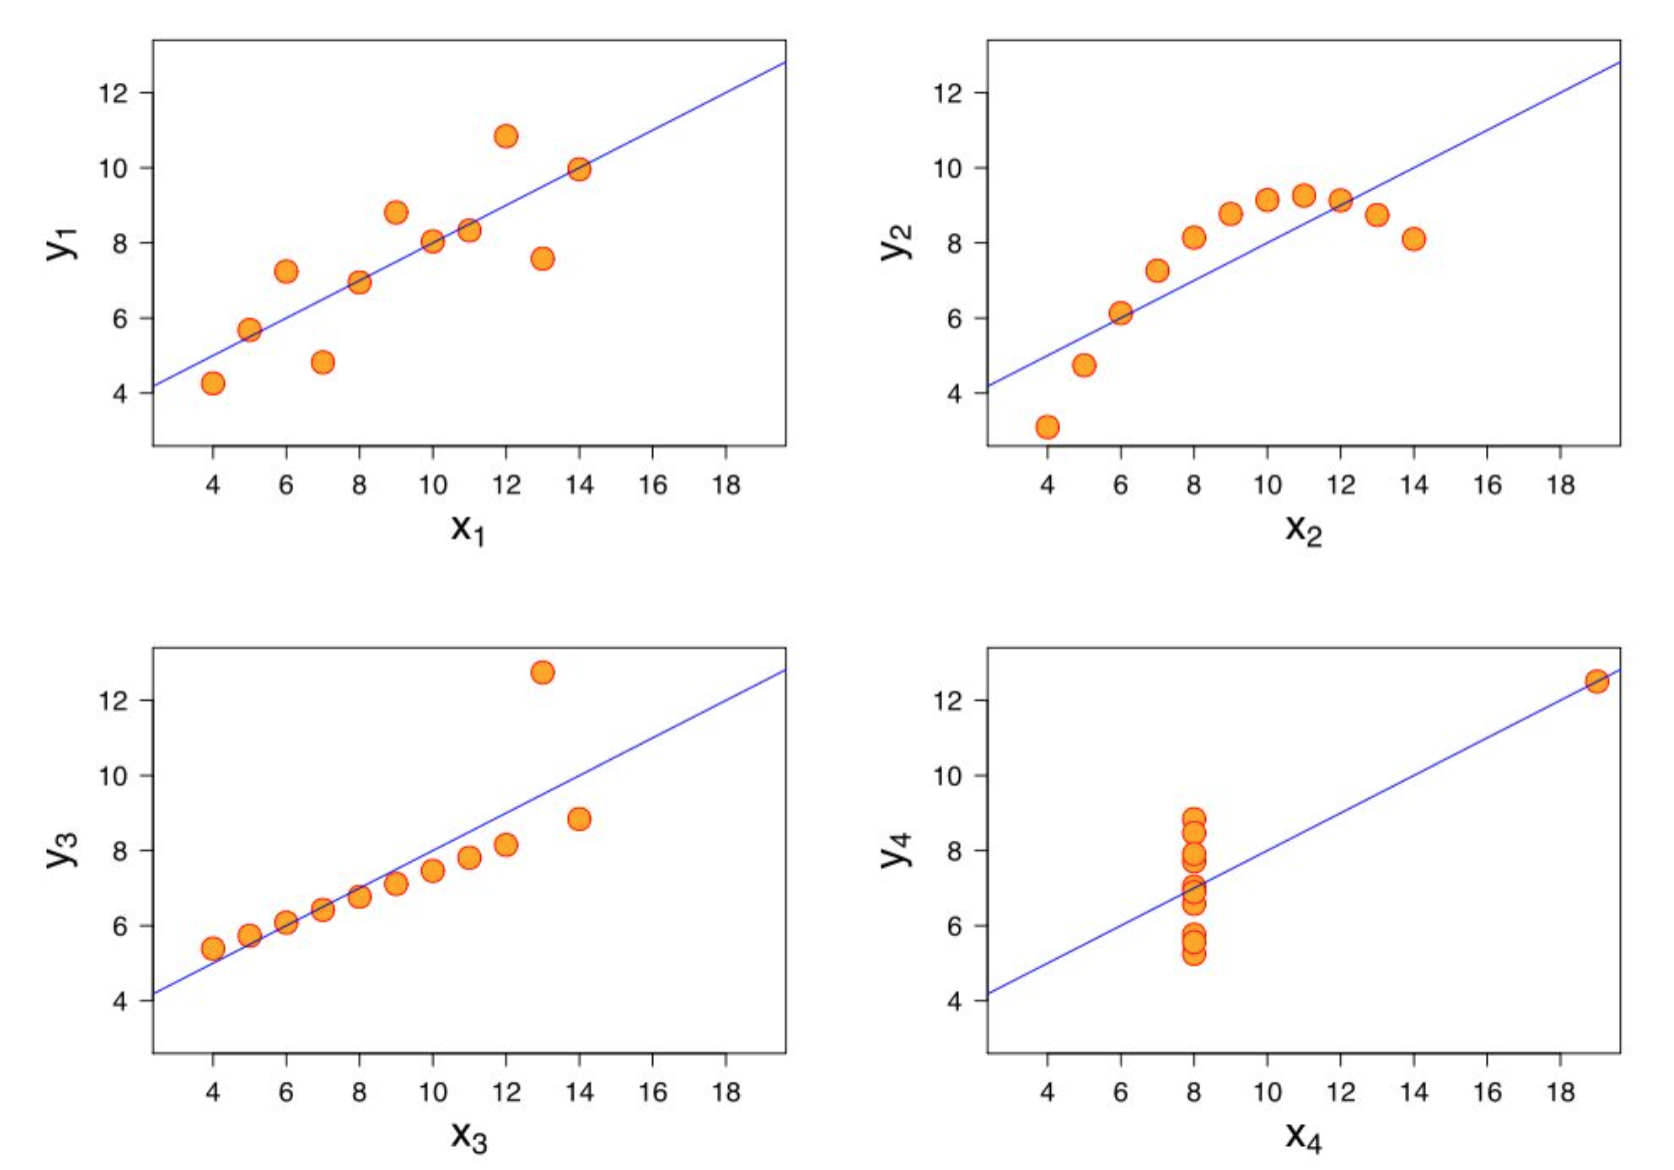
\includegraphics[width=10cm]{./img/05/anscombe}
 \caption{\label{pic:anscombe} Anscombe's quartet}
\end{figure}

%================ Simpson paradox =================
\subsubsection{Simpson's paradox: aggregation of data}

\textbf{Certain tendencies can appear, disappear or even reverse themselves when aggregating the data!} This was the case when media started blaming Berkey of being unfair with women applications (looking at left table of FIG \ref{pic:Berkley}). After further investigation (and de-aggregation of the data), it appeared that at the opposite... Berkeley was unfair with men! (Right table of the same FIG).

This paradox comes from the fact that women (according to these tables) tended to apply for more competitive departments, with lower rates of admission. \textbf{When aggregating the data, we lost this subtlety and then draw a wrong conclusion.} 

Simpson's paradox can appear in a lot of cases and can be very hard to detect. The \href{https://en.wikipedia.org/wiki/Simpsons_paradox}{wikipedia page of Simpson's paradox} describes a lot of examples and, for the ones interested, a great book relates lots of statistical errors that drove to miscarriages of justice: \href{https://books.google.ch/books/about/Math_on_Trial.html?id=PFAIb6FTgY4C&source=kp_cover&redir_esc=y&hl=fr}{Leila Schneps and Coralie Colmez, Math on Trial: How Numbers Get Used and Abused in the Courtroom} 

\begin{figure}[h]%---------------FIG--------------
 \centering
 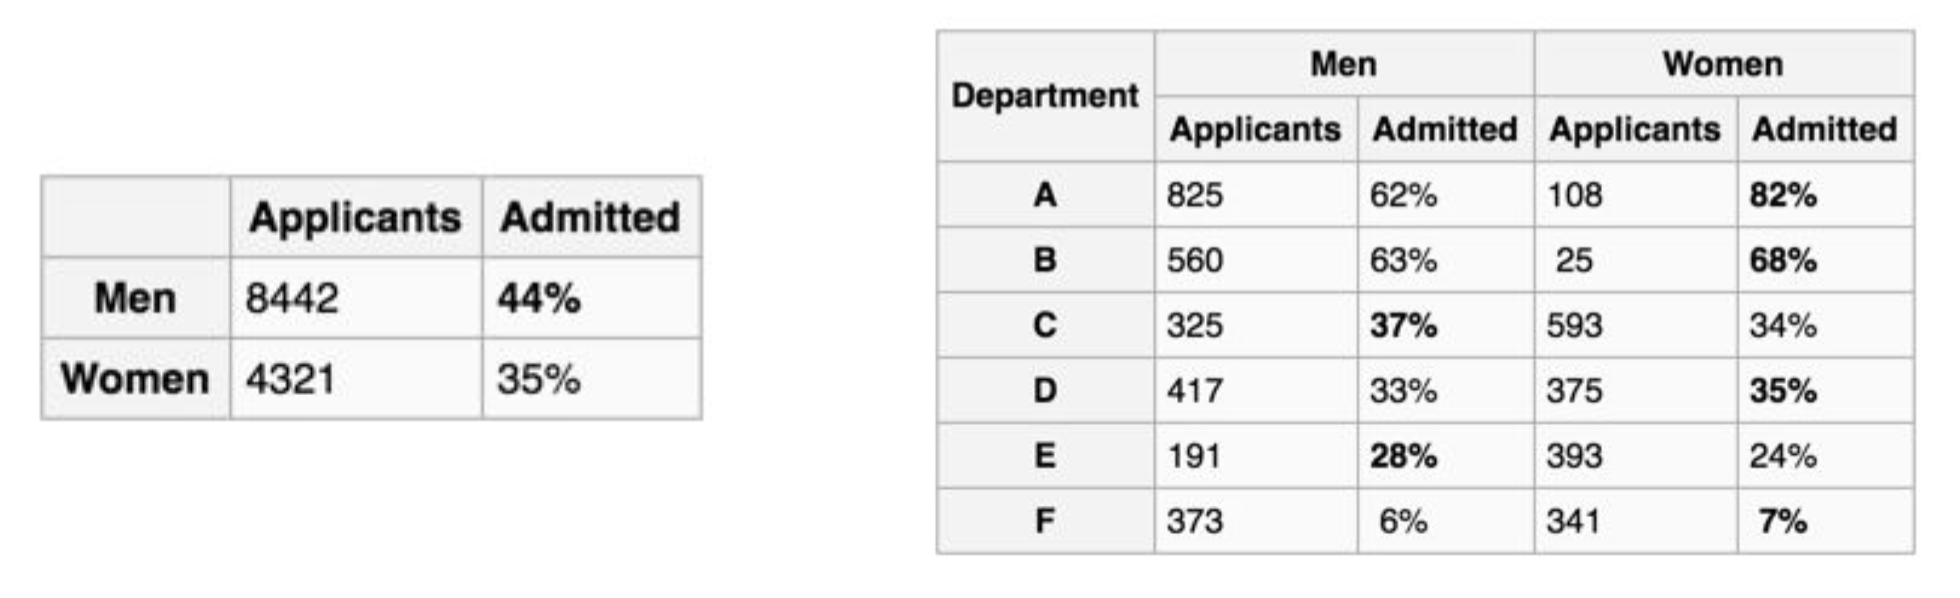
\includegraphics[width=10cm]{./img/05/Berkeley}
 \caption{\label{pic:Berkley}Berkley admission tables of 1973}
\end{figure}

% ================ Basic stats ==============
\subsection{Refresh of basic statistics concept}

\begin{itemize}
	\item {\bf Probabilities}: mathematical theory that describes uncertainty. \\
	\item {\bf Statistics}: Set of techniques for extracting useful info from data
\end{itemize}

\begin{framed}
{\it {\bf Probability and Statistics} are related areas of mathematics which concern themselves with analyzing the relative frequency of events. Still, there are fundamental differences in the way they see the world:\\
\textbf{Probability deals with predicting the likelihood of future events}, while \textbf{statistics involve the analysis of the frequency of past events}. \\  
Probability is primarily a theoretical branch of mathematics, which studies the consequences of mathematical definitions. Statistics is primarily an applied branch of mathematics, which tries to make sense of observations in the real world.}
\signed{\href{http://www3.cs.stonybrook.edu/~skiena/jaialai/excerpts/node12.html}{Steven S. Skiena, "Calculated Bets", Cambridge University Press, 2001}}
\end{framed}

% ================ Bayes Theorem ==============
\subsubsection{Bayes Theorem}
The theorem express the very intuitive statement that:

{\it The probability of observing event A and B is the probability of observing B multiplied by the probability of observing A knowing that B occurred.}

Mathematically it's expressed as: 
\be
P(A\vert B)P(B)=P(A\cap B)=P(B\vert A)P(A)
\ee
Or equivalently
\be
P(A|B)={\frac  {P(B|A)P(A)}{P(B)}}
\ee

More about Bayes Theorem on \href{https://en.wikipedia.org/wiki/Bayes_theorem}{wikipedia}.

% ================ Random Variables ==============
\subsubsection{Random Variables}
A \textbf{random variable} is a quantity that can take various values, each one associated with a probability of apparitions. The some of these probabilities will always be 1.
\be
X\colon \Omega \to E
\ee

$\Omega$ being a probability space and $E$ a measurable space (usually $E = \mathbb{R}$).

Any random variable can be described by its \href{https://en.wikipedia.org/wiki/Cumulative_distribution_function}{cumulative distribution function}, which describes the probability that the random variable will be less than or equal to a certain value.

Two \textbf{independent variables} are defined as
\be
{\mathbb  {P}}(A\cap B)={\mathbb  {P}}(A)\cdot {\mathbb  {P}}(B).
\ee
or equivalently (by Bayes Theorem)
\be
\label{indep}
{\mathbb  {P}}(A\mid B) =  {\mathbb  {P}}(A)
\ee

More about Bayes Theorem on \href{https://en.wikipedia.org/wiki/Random_variable}{wikipedia}.

% ================ Law of Large Number ==============
\subsubsection{Law of Large Numbers}

The Law of Large Numbers links, in some way, the probability to the statistics. It's, again, a very intuitive statement, even if not so easy to prove (as always in mathematics).

\begin{framed}
In probability theory, the\textbf{ law of large numbers} (LLN) is a theorem that describes the result of performing the same experiment a large number of times. According to the law, \textbf{the average of the results obtained from a large number of trials should be close to the expected value}, and will tend to become closer as more trials are performed.
\signed{\href{https://en.wikipedia.org/wiki/Law_of_large_numbers}{Wikipedia}}
\end{framed}

A common mistake is to deduce that, in the case of playing heads or tails for example, observing a lot of time \textbf{heads} increase the probability of observing \textbf{tails}. This is absolutely wrong. The variables are perfectly independent and, according to Eq \ref{indep}, the probability stays exactly 50\%. This is the perfect example of confusing probabilities with statistics.

% ================ CLT ==============
\subsubsection{Central Limit Theorem}

\textbf{Central Limit Theorem} states that the mean of independent and identically-distributed random variables will converge to \textbf{Gaussian Distribution} (Normal Distribution).

% ================ CLT ==============
\subsection{Most common distributions}

\begin{itemize}
	\item \textbf{Gaussian Distribution} (fig \ref{gauss}) results from independent and identically-distributed variables 
	$f(x\;|\;\mu ,\sigma ^{2})={\frac {1}{\sqrt {2\sigma ^{2}\pi }}}\;e^{-{\frac {(x-\mu )^{2}}{2\sigma ^{2}}}}$
	\href{https://en.wikipedia.org/wiki/Gaussian_distribution}{More on wikipedia}
	
	\item \textbf{Poisson Distribution} (fig \ref{poisson}) describe the observation of events happening in a delimited time-laps. E.g: an event happens in average 4 times each 10 minutes ($\lambda = 4$). What's the probability that it appears after only 3 times in this same interval ($k = 3$)? $p(k) = \frac{\lambda ^k}{k!}e^{-\lambda}$ \href{https://en.wikipedia.org/wiki/Poisson_distribution}{More on wikipedia}

	\item \textbf{Exponential Distribution} (fig \ref{exp}) describes the time between two events in a Poisson process. $P(x) = \lambda e^{- \lambda x}$ \href{https://en.wikipedia.org/wiki/Exponential_distribution}{More on wikipedia}
	
	\item \textbf{Binomial Distribution} (fig \ref{binomial}) describes the discrete distribution on success in a yes/no experiment. (E.g. coin tossing or any win/lose game). $f(k;n,p)=\Pr(X=k)={\binom {n}{k}}p^{k}(1-p)^{n-k}$ \href{https://en.wikipedia.org/wiki/Binomial_distribution}{More on wikipedia}
	
	\item \textbf{Multinomial Distribution} generalizes Binomial law. \href{https://en.wikipedia.org/wiki/Multinomial_distribution}{More on wikipedia}
	
	\item \textbf{Zipf Distribution} is an empirical discret description of word frequency in a text. \href{https://en.wikipedia.org/wiki/Zipfs_law}{More on wikipedia}
	
	\item \textbf{Pareto Distribution} is the equivalent of Zipf in a continuous space. It allows, amongst other things, to give a theoretical base of the "80-20 principle" (20\% of the causes produce 80\% of the effects). \href{https://en.wikipedia.org/wiki/Pareto_distribution}{More on wikipedia}
	
	\item \textbf{Yule-Simon distribution} describes discret frequencies of term too. \href{https://en.wikipedia.org/wiki/Yule?Simon_distribution}{More on wikipedia}
\end{itemize}

{\bf \color{red}  You should understand the distribution of your data before applying a model!}

\begin{figure}[H] %----------- SubGraph ---------------------
\centerline{
\subfigure[Probability density function] {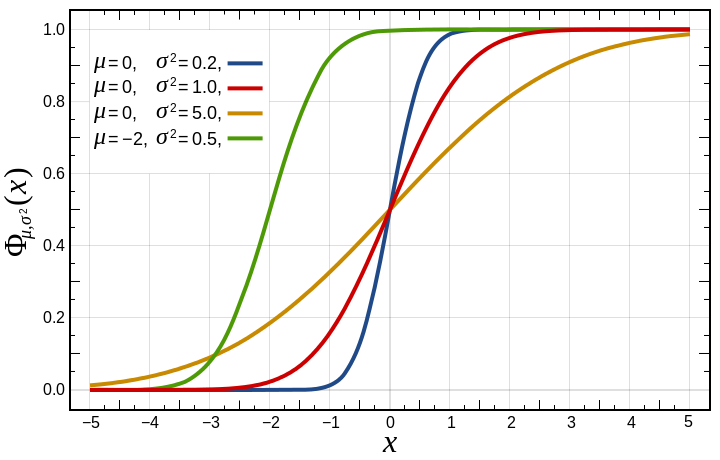
\includegraphics[width=5.5cm]{img/05/gauss_density}}
\subfigure[Cumulative distribution function] {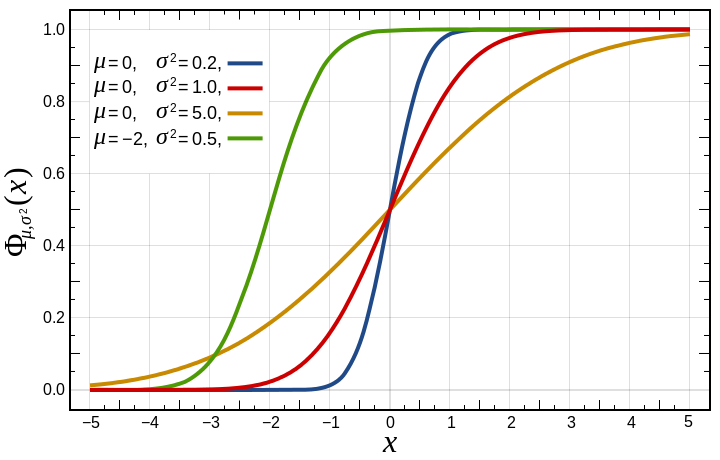
\includegraphics[width=5.5cm]{img/05/gauss_cumul}} 
}
\caption{\label{gauss} 
Gaussian distribution 
} 
\centerline{
\subfigure[Probability density function] {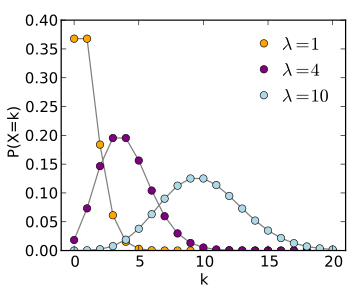
\includegraphics[width=5.5cm]{img/05/Poisson_pmf}}
\subfigure[Cumulative distribution function] {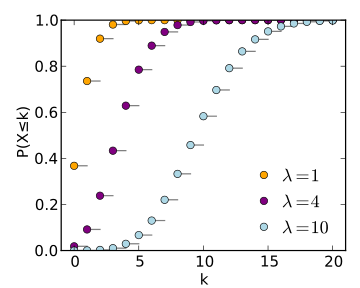
\includegraphics[width=5.5cm]{img/05/Poisson_cdf}} 
}
\caption{\label{poisson} 
Poisson distribution 
}
\centerline{
\subfigure[Probability density function] {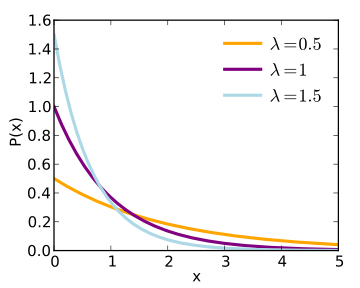
\includegraphics[width=5.5cm]{img/05/exp_pmf}}
\subfigure[Cumulative distribution function] {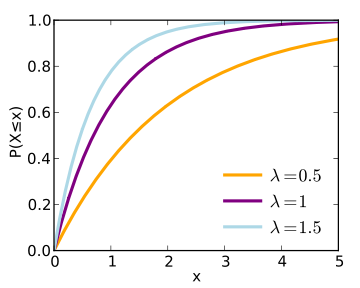
\includegraphics[width=5.5cm]{img/05/exp_cdf}} 
}
\caption{\label{exp} 
Exponential distribution 
} 
\centerline{
\subfigure[Probability density function] {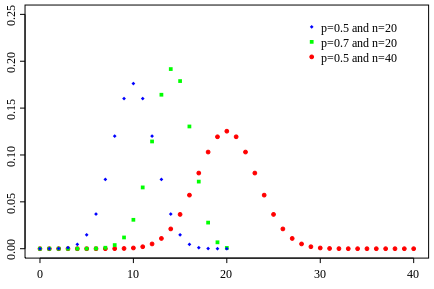
\includegraphics[width=5.5cm]{img/05/binomial_pmf}}
\subfigure[Cumulative distribution function] {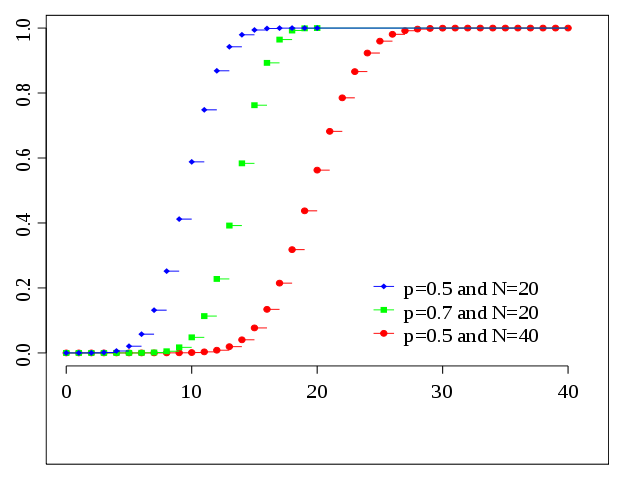
\includegraphics[width=5.5cm]{img/05/binomial_cdf}} 
}
\caption{\label{binomial} 
Binomial distribution 
} 
\end{figure}



% ================ Measurement ==============
\subsection{Measurement on Samples}

In practice, we (almost) never analyse the entire population. We always work on a subset of it called \textbf{sample}. The \textbf{variance} is the variation between elements of our sample, that we hope to be the same as the population. The \textbf{biases} is the systematic variation between the entire population and the sample we chose.

When randomly select elements of the population to be part of the sample, we have a great chance that the bias is small (i.e. that the distribution of the sample corresponds to the distribution of the population). But do not forget that there is a probability (even if a small one) to select elements that \textbf{biased our measures}! This probability can even increase when you clean the data, if you don't do it wisely.

A stupid example could be a study on population education in which, during the cleaning, you remove the answers containing misspelling. Uneducated people are more likely to commit misspelling so, removing them, you artificially biais the sample.

% ================ Test Statistic ==============
\subsection{Test Statistic}

(The only good and easy-to-understand explanation about test statistics I ever found is available on \href{http://hamelg.blogspot.ch/2015/11/python-for-data-analysis-part-24.html?view=flipcard}{hamelg.blogspot})

The idea behind test statistics is \textbf{instead of proving that our assumption is true, let's calculate the probability that our observations occur by chance (null hypothesis or $H_0$). If this probability is very low, then there is a good chance that our hypothesis is true!}

The probability that this happens by chance is called $pvalue$ and we usually consider that if $pvalue \leq 0.05$ our hypothesis is true ($pvalue \leq 0.01$ in some strict cases).

% ================ Test Statistic ==============
\subsubsection{Example with t-test}

Let's take the example on FIG \ref{pic:ttest}. The \textbf{Null Hypothesis} $H_0$ represents the distribution of observation we can do, assuming there is no correlation between the values we measured. The \textbf{Alternative} is $H_A$, our hypothesis which states that, at the opposite, there is correlations.
\begin{itemize}
	\item If the observation we test is $x=3$, there is \textbf{less than 5\% probabilities that it was produced by $H_0$} ($pvalue \leq 0.05$). Our hypothesis $H_A$ is considered true.

	\item If the observation we test is $x=0$, there are \textbf{more than 5\% probabilities that it was produced by $H_0$} (more or less 40\%). Our hypothesis $H_A$ is considered false.
\end{itemize}

{\color{red} An important thing to notice is that \textbf{it does not provide the truth on statistic}, it only provides information about how likely is the null hypothesis! Let's look back to the example}

\begin{itemize}
	\item The $x=3$ observation \textbf{could have been produced by the red area}, meaning that it's part of the small 5\% chance of being produced by the $H_0$. The test will say that our hypothesis is true, which will be a \textbf{false positive}.

	\item The $x=0$ observation \textbf{could have been produced by the blue area}, meaning that even it $H_0$ have great chance to produce it, it was in fact produced by $H_A$.  The test will say that our hypothesis is false, which will be a \textbf{false negative}.
\end{itemize}

\begin{figure}[h]%---------------FIG--------------
 \centering
 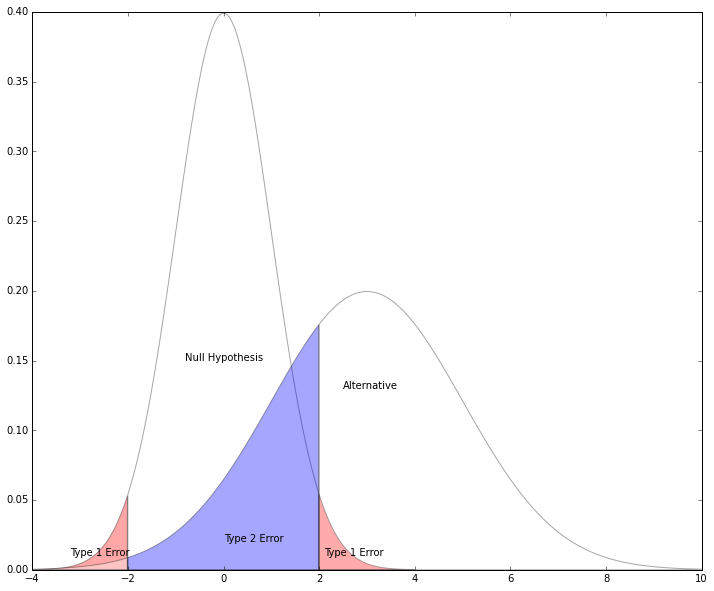
\includegraphics[width=10cm]{./img/05/t-test}
 \caption{\label{pic:ttest} T-Test example}
\end{figure}

% ================ Test Statistic ==============
\subsubsection{Choose the right test}

A lot of tests exist and we must choose wisely which one to use, according to data and hypothesis characteristics. FIG \ref{pic:testtree} show a decision tree helping to choose the test which suits best our situation.

\begin{itemize}
 \item Question ? 
 \item Data type ?
 \item Sample size
 \item Variance known? 
 \item Variance of several groups equals?
 \item ...
\end{itemize}

\begin{figure}[h]%---------------FIG--------------
 \centering
 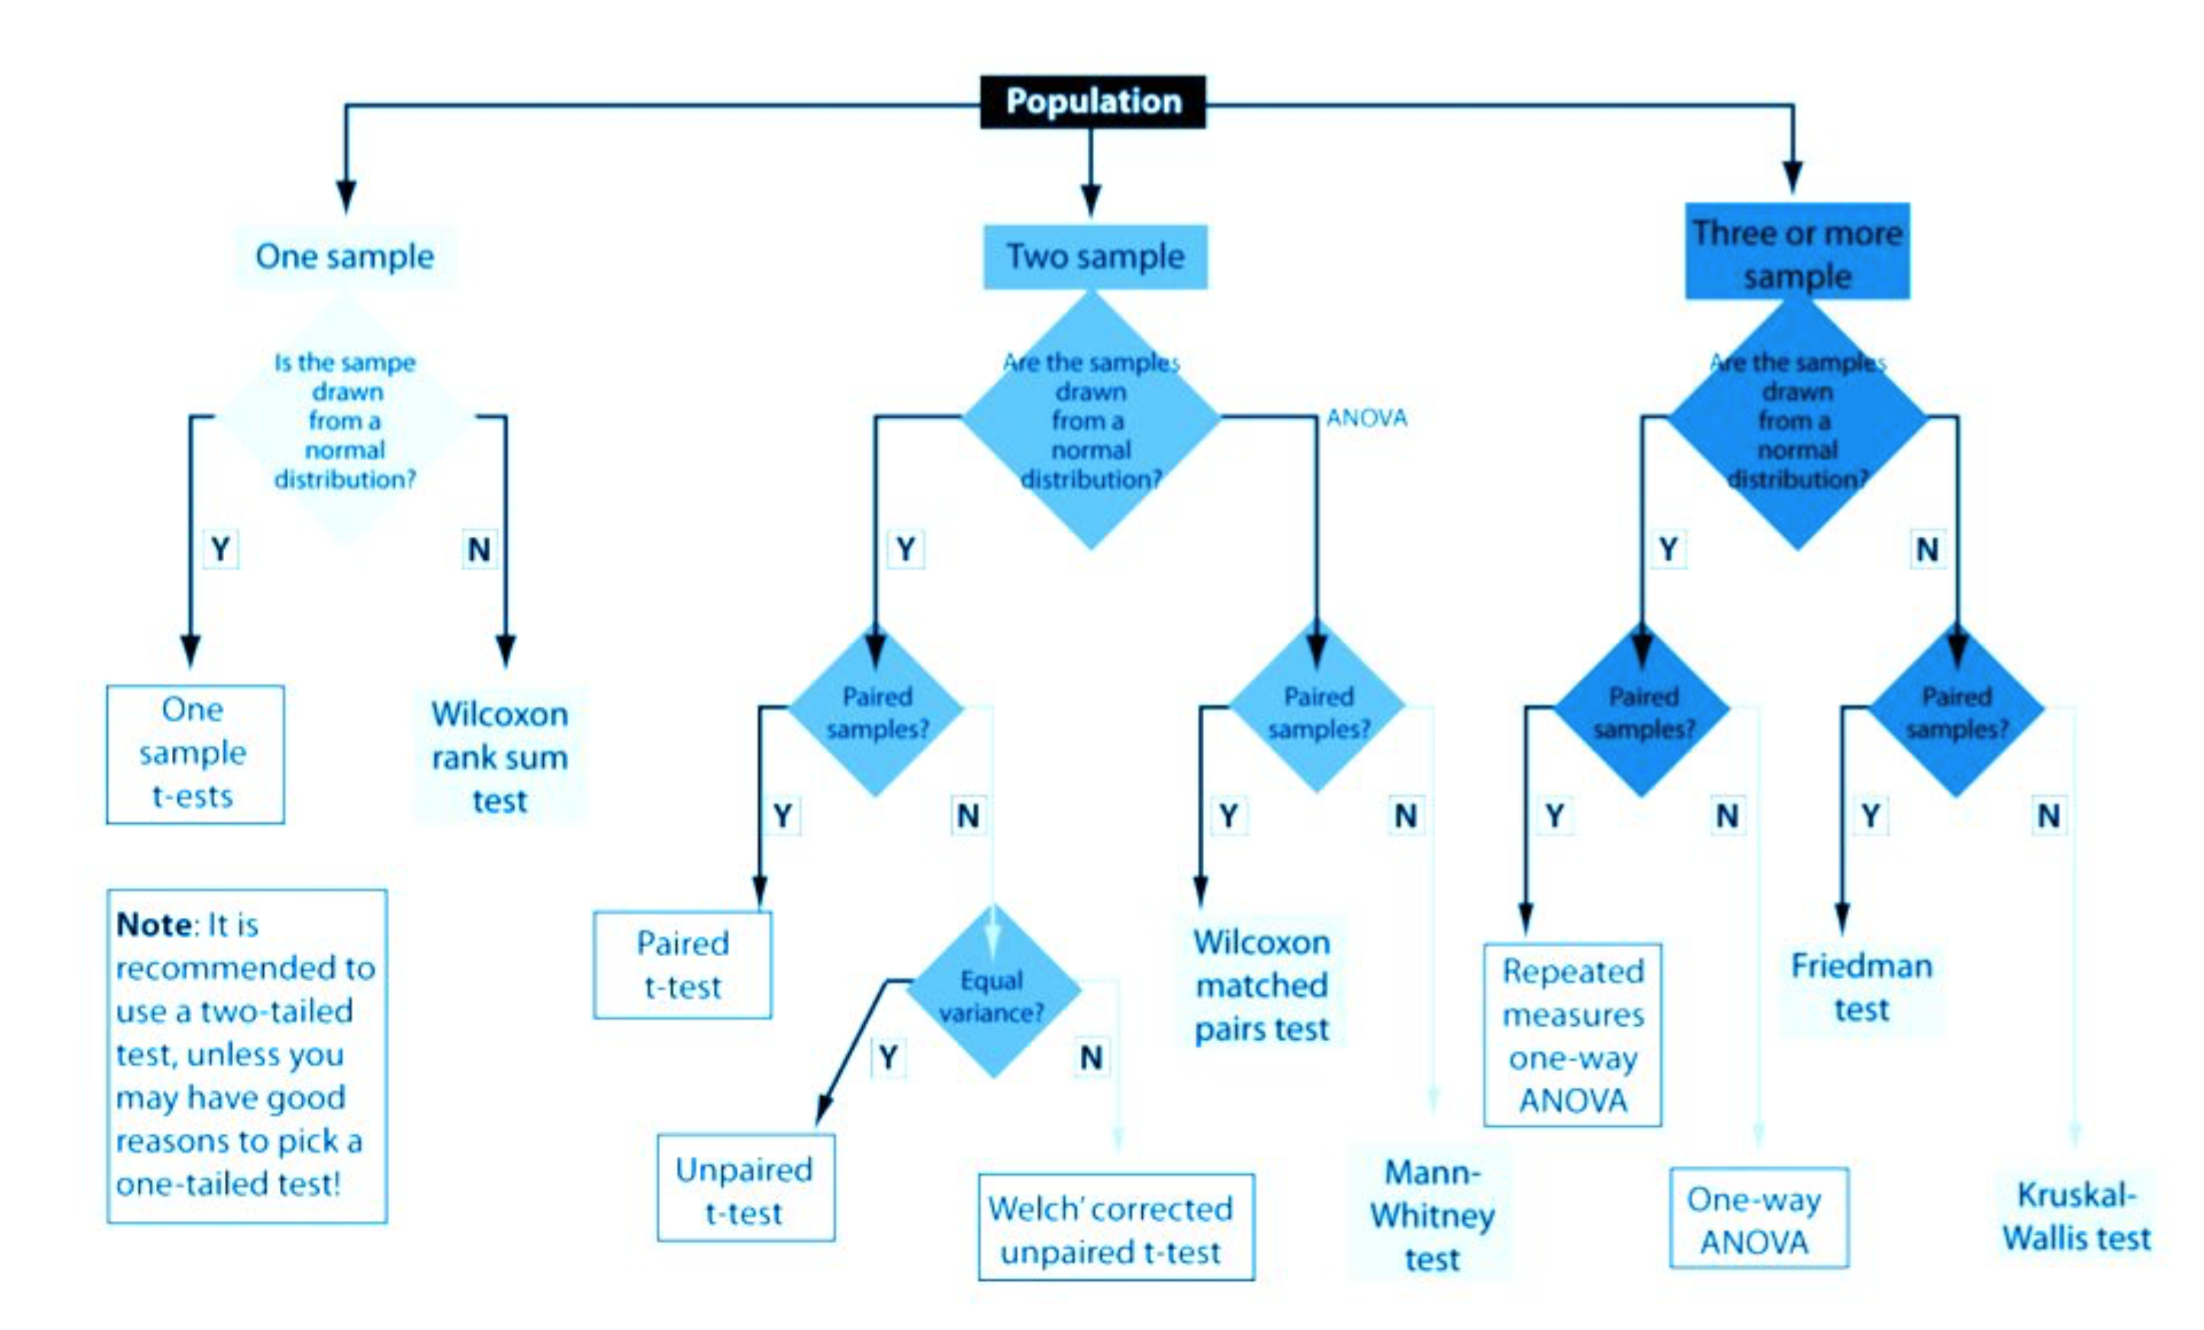
\includegraphics[width=15cm]{./img/05/choose_test}
 \caption{\label{pic:testtree} Statistical test decision tree}
\end{figure}


% ============================================
\subsubsection{Family-wise Error}

Following this simple math equation, we can figure out that the more experiment we do to test the hypothesis, the more likely we are to find that one of them are spuriously right! This is because the reverse point of view of the test. We are testing the fact that $H_0$ is unlikely, not directly that $H_A$ is likely. 

\begin{equation} \label{eq1}
\begin{split}
P(false \: positive) &= \alpha = 0.05 \\ 
P(true \: positive) &= 1 - \alpha = 0-95 \\
P(true \: positive \: on \: each \: experiment) &= (1 - \alpha)^k \\
P(at \: least \: on \: false \: positive \: on \: one \: experiment) &= 1 - (1 - \alpha)^k
\end{split}
\end{equation}

To counter that, two possible correction exists
\begin{itemize}
  \item Bonferroni correction : $\alpha_c = \frac{\alpha}{k}$ 
  \item Sidak correction: $\alpha_c = 1- (1 - \alpha)^{1/k} $
\end{itemize}


% ============================================
\subsubsection{Non-Parametric tests}

All the tests so fare assume that the data are {\bf normally distributed} and that the samples are {\bf independent of each other and all have the same distribution.} (IID) They may be inaccurate if those assumptions are not met. Therefore, make sure the data satisfy the assumptions of the test we're using. Watch out for:
\begin{itemize}
 \item \textbf{Outliers} will corrupt many tests that use variance estimates.
 \item \textbf{Correlated values as samples}, e.g. if you repeated measurements on the same subjective
 \item \textbf{Skewed (bias) distributions} give invalid results.
\end{itemize}

Some tests make no assumptions and thus can be used on very general cases: \textbf{K-S test}, \textbf{Permutation test} and \textbf{Bootstrap confidence interval}.


%================================================
\subsubsection{K-S test}
K-S (Kolmogorov-Smirnov) test is a very useful test for checking whether two (continuous or discrete) distributions are the same. 
\begin{itemize}
 \item In the {\bf one-sided test}, an observed distribution (e.g. some observed values or a histogram) is compared against a reference distribution (e.g., power-law).
 \item In the {\bf two-sided test}, two observed distributions are compared.
 \item The K-S statistic is just the {\bf max distance between the CDFs} (Cumulative Distribution Function) of the two distributions.
 \item The K-S test can be used to test {\bf whether a data sample has  a normal distribution} or not.
 \item Thus it can be used as a sanity check for any common parametric test (which assumes normally distributed data).
 \item It can also be used to compared distributions of data values in large data pipeline: {\bf Most errors will distort the distribution of a data parameter and a K-S test can detect this.}
\end{itemize}
This test is expensive! Check for more information on the \href{https://en.wikipedia.org/wiki/Kolmogorov?Smirnov_test}{wikipedia page}.

\clearpage
% !TEX root = ../notes.tex

% ================  (Interactive) Visualization ==============

\section{Data Visualization}
\subsection{Two main purposes}

In this chapter we are going to talk about visualization in general and then about what it is called interact visualization. The first thing we do when we talk about visualization is to split it into two different tracks. 

\begin{itemize}
\item {The first one is about \emph{analysis}: you want to support reasoning about information. For instance, when you have a \texttt{DataFrame} you can make a plot of the distribution of the attribute in order to identify outliers, missing data and \emph{so forth}. In general with this kind of visualization you can do more like discover structures, quantify values and influences.
\emph{This way of using visualization is extremely important for debugging purposes}.}

\item{The second  is the \emph{communication} part and it is about informing and persuade people.  The key difference in working in \emph{Data Science} and exclusively in \emph{Machine Learning} or \emph{Statistics} is the fact that you don't just stop after getting a good model and evaluating its accuracy. You would make a story that you convey to people.
For this reason we have to use visualization that can capture attention, can engage people and can tell a story visually (tell a story using visual tools takes a lot less time) and last but not least, you are focused only on certain aspects omitting others. It is a double edge sword. That is because, on one hand you have to consider that there is an information overflow that people are suffering in general (we get too many media in which we consume information) so we do not want our visualization conveys more information than  a human being can actually get in a few seconds). On the other hand, we have to do it carefully, avoiding omitting some information just because difficult to handle or with, apparently, nonsense.}
\end{itemize}

\subsection{Data exploration}

In order to do a good \emph{Data exploration} analysis by means of visualization:

\begin{itemize}
\item {Get familiar with your favorite graphing package:}
\begin{itemize}
\item \texttt{Matplotlib} which is widely used in \texttt{Python}
\item \texttt{Seaborn} and \texttt{Bokeh} that are two additions on top of \texttt{Matplotlib}
\item \texttt{D3.js} (\texttt{Javascript}) is the most famous framework for interactive graphics
\end{itemize}
\item {Get fluent with plotting:}
\begin{itemize}
\item Histograms
\item Scatter plots
\item Line and bar plots
\end{itemize}
\end{itemize} 

\subsubsection{One variable}

Whenever we want to look at the data we can use histograms, they tell us a lot about the single variable. Once you plot them, you can try to figure out their distribution, for instance we can identify skewed distributions, multimodal or long tail data. 

\begin{figure}[H]%---------------FIG--------------
 \centering
 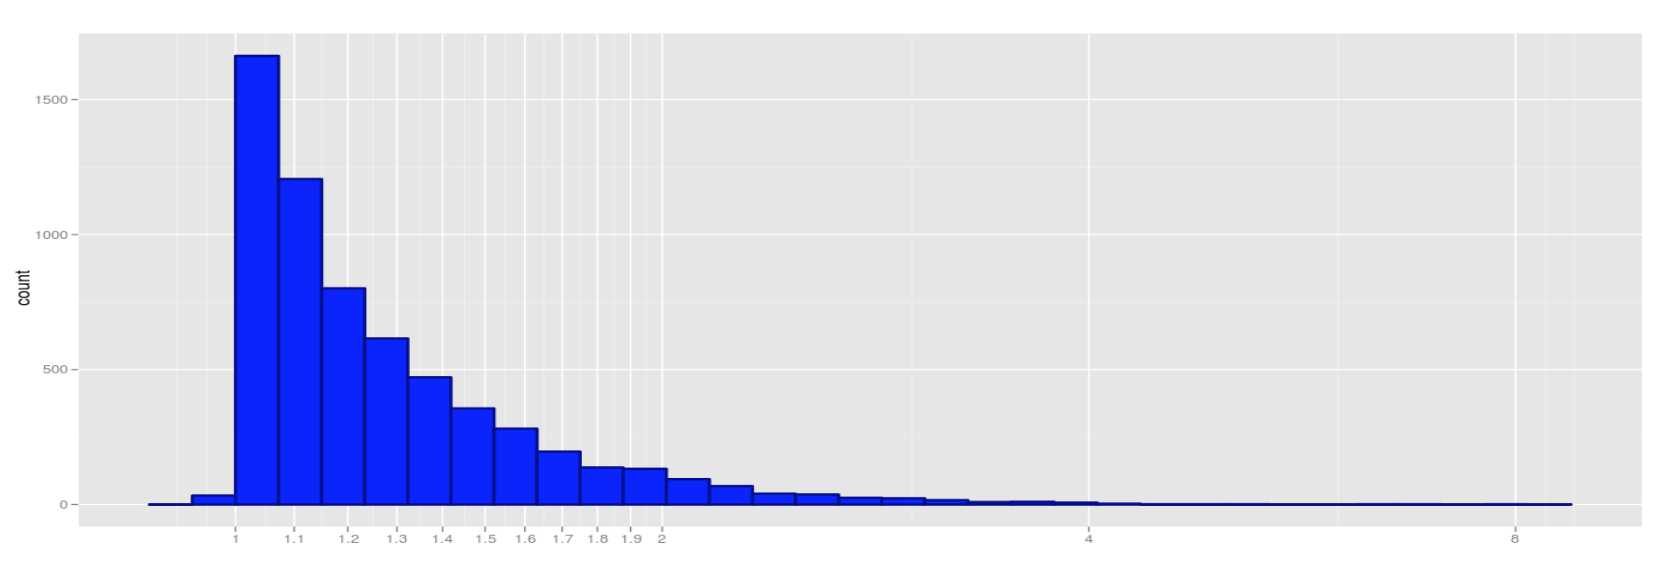
\includegraphics[width=13cm]{./img/06/long_tail}
 \caption{\label{pic:long_tail} Example of long tail data.}
\end{figure}

The latter is characterized by a bunch of bins that reveal a lot of occurrences and bars in the tail where we observe a very few occurrences. Many of this long tail data follow a \href{https://en.wikipedia.org/wiki/Power\_law\#Power-law\_probability\_distributions}{\emph{power-law}}. To claim the latter we need to run some test on data that proofs the statistical significance of our hypothesis, otherwise we can just state that it looks like a \emph{power-law}. For a graphical representation:

\begin{enumerate}
\item Sort the histogram counts by magnitude, descending.
\item Plot count vs bucket number on a log-log plot.
\end{enumerate}


\begin{figure}[H]%---------------FIG--------------
 \centering
 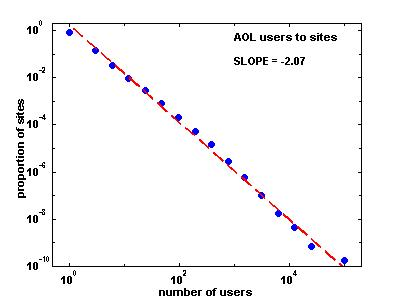
\includegraphics[width=13cm]{./img/06/power_law}
 \caption{\label{pic:power_law} Example \href{https://en.wikipedia.org/wiki/Zipf\%27s\_law}{power law}.}
\end{figure}


Generally this law is characteristic of social-influence processes, to know more look up for \emph{Preferential attachment}.

The \emph{multinomial} data registers more than one peak in the histogram, it suggests that there are two or more distinct populations of a sample. When you deal with something like this do not guess! Explore further by using, e.g., color and a histogram of multiple populations. 


\begin{figure}[H]%---------------FIG--------------
 \centering
 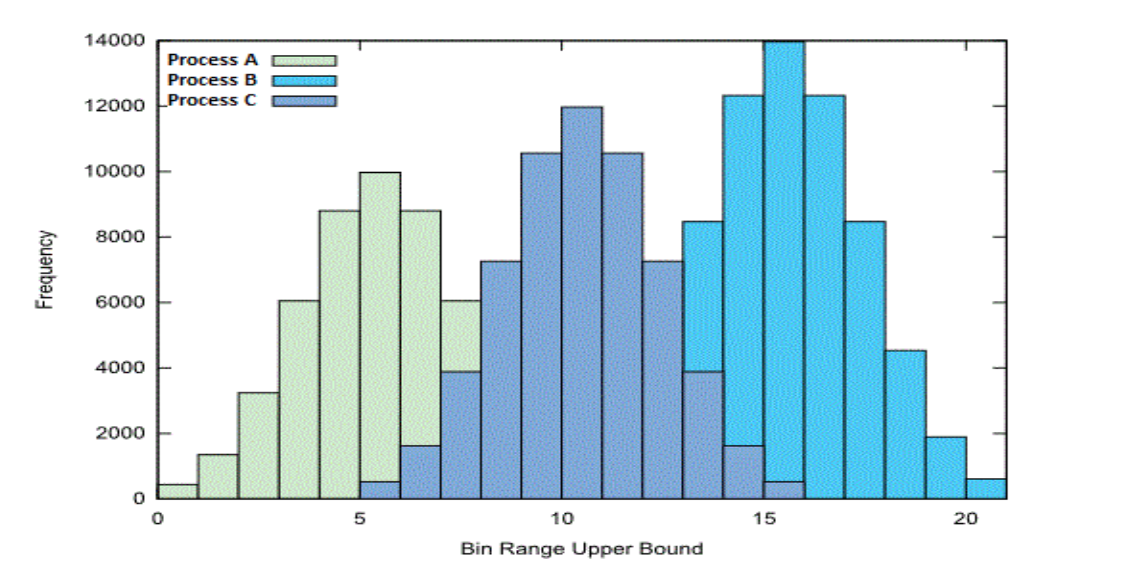
\includegraphics[width=13cm]{./img/06/multimodal}
 \caption{\label{pic:multimodal} Example of multimodal data.}
\end{figure}


Sometimes data is weird and is very hard to explain. Also in this case, do not guess! Trace through the data pipeline to find where the strangeness comes from. Usually it is a processing bug. Hence, check your code!

There is a way for a \emph{proactive Weird data Detection}. If data looks normal, take a picture and save it for later, then periodically compare new data with old whenever there is a pipeline update. Generally always try to have a theory of what the data should look like!

\subsubsection{More than one variable}
 
Most of the time we are interested in visualizing more than one variable, here a \emph{non-thorough} list of possibilities is listed:

\begin{itemize}
\item Two variables 
\begin{itemize}
\item \emph{Scatter plots} quickly expose the relationships between two variables
\end{itemize} 
\item  More than two variables
\begin{itemize}
\item \emph{Stacked plot}: stack variable is discrete, useful to explore data (Figure \ref{pic:stacked})
\begin{figure}[h]%---------------FIG--------------
 \centering
 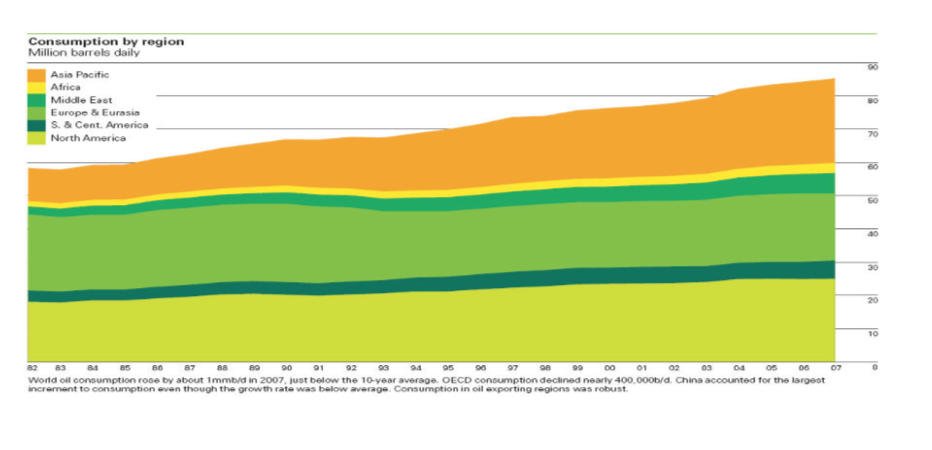
\includegraphics[width=13cm]{./img/06/stacked}
 \caption{\label{pic:stacked} Example of stacked plot.}
\end{figure}
\item \emph{Parallel coordinate plot}: one discrete variable, an arbitrary number of other variables (when this number increases it risks becoming very messy), see an example in Figure \ref{pic:parallel}
\begin{figure}[h]%---------------FIG--------------
 \centering
 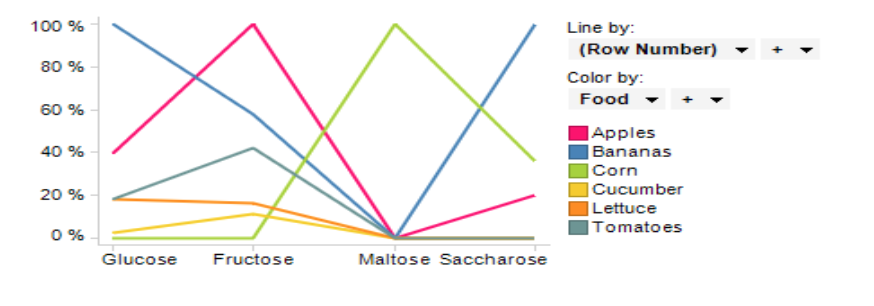
\includegraphics[width=13cm]{./img/06/parallel}
 \caption{\label{pic:parallel} Example of parallel plot.}
\end{figure}
\item \emph{Radar Chart}: one discrete variable (through the radar design), an arbitrary number of other variables (Figure \ref{pic:radar})
\begin{figure}[h]%---------------FIG--------------
 \centering
 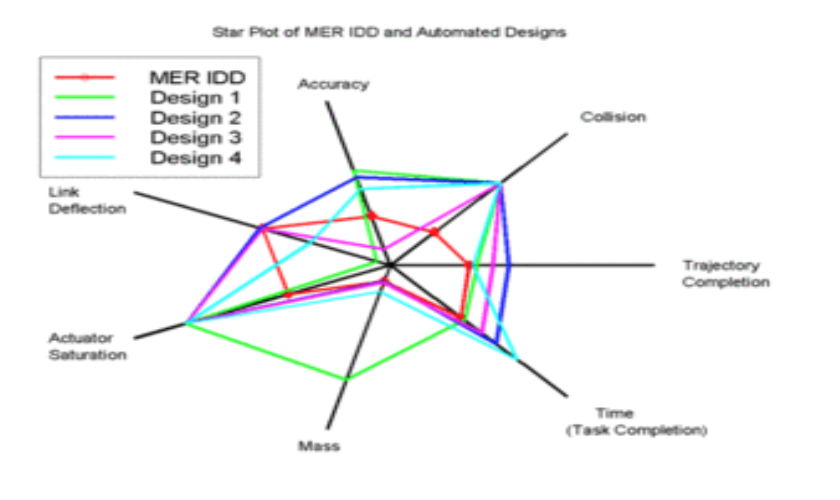
\includegraphics[width=13cm]{./img/06/radar}
 \caption{\label{pic:radar} Example of radar plot.}
\end{figure}
\end{itemize}
\end{itemize}


When you deal with a high number of variables, a valid idea to visualize in a better way is to reduce the number of variables applying algorithms, this pocess is called \emph{Dimensionality reduction}, one example is the \href{https://en.wikipedia.org/wiki/Principal\_component\_analysis}{ \emph{PCA}}. Intuitively, given twenty different variables, many tend to not variate a lot, \emph{PCA} extracts the couple of attributes that really make the difference allow visualization of high-dimensional continuous data in 2D using principal components. Hence, instead of directly plot multivariate data, try to think whether a dimensionality reduction can be useful.

We argued for analysts is important to form expectations of what the data should look like. This helps against pipeline errors and to identify interesting patterns. But beware of seeing \href{https://en.wikipedia.org/wiki/Martian1_canal}{\emph{Martian Canals}}: do not see things that are not there. Moreover, an observer should also be attuned to patterns that are not part of his theory, in other words, to expect the unexpected. 


\subsection{Moving Towards Interactive Viz}

Interactive visualization is a new field and it's getting more and more common. Our aim is to deliver results and this has been enabled by the new web technologies and in general by few frameworks essential for the current state of the art. \texttt{JavaScript} plays a very important role in the field. The vast majority of the libraries that allow to do visualization are in \href{https://www.codecademy.com/learn/javascript}{\texttt{JavaScript}}, so if you know how to use it or if you want to learn how to use it, it is definitely a good tool to have in your toolbar. 

A visualization is worth a thousand words! Representing in 2D more than two variables has been being a challenge since a long time ago. Even without the help of the machines, someone tried to do something in \href{https://en.wikipedia.org/wiki/Charles\_Joseph\_Minard}{this} field. Nowadays the technology allows the \emph{researchers} to go further and to use all their creativity and skills, nevertheless so many efforts should be put in. Lots of concepts have been developed and, for those interested, there are pioneers of the field that should be taken into \href{https://en.wikipedia.org/wiki/Edward\_Tufte}{consideration}.

As we already said the visualization has the characteristic of engaging the audience easily and it often results clear and understandable (be careful, not all the graphs and representations you look at are reliable, fair and proper!!). Hence it can be used to globally describe \href{https://www.ted.com/talks/hans\_rosling\_shows\_the\_best\_stats\_you\_ve\_ever\_seen}{phenomena} not easy to understand otherwise. Today, many are the \href{https://www.gapminder.org/tools/#\_chart-type=bubbles\&state\_time\_end=2015;\&entities\%2F\_minimap\_show\_geo.cat@=main\%2F\_religion\%2F\_2008;;;\&marker_color\_which=geo.main\%2F\_religion\%2F\_2008}{websites} where you can play with data using visualization.

Visualizing data is becoming a new way to spread information. More than ever, we recognize the existence of \emph{Data journalism}, more data are available, many people have programming skills. Thus, it is simple to find persons who combine both writing and programming skills. There are journals that stand out, such the \href{http://www.nytimes.com/interactive/2014/06/05/upshot/how-the-recession-reshaped-the-economy-in-255-charts.html?\_r=0}{\emph{New York Times}}, \emph{Forbes} and \emph{The Economist}. They build up teams of researchers who are the best experts in the field. Hence, they can be considered a great source of best practices in viz.

\subsection{Visualization definitions}

There is not a unique way to define visualization, here some definitions that try to include many few aspects are listed:

\begin{itemize}
\item \emph{Transformation of the symbolic into the geometric} (McCormick et al. 1987) 
\item \emph{... finding the artificial memory that best supports our natural means of perception.} (Bertin 1967)
\item \emph{The use of computer-generated, interactive, visual representations of data to amplify cognition.} (Card, Mackinlay \& Shneiderman 1999) 
\end{itemize}

\subsection*{The 10 rules}

When you do visualization you have to take care of the following \href{http://www.sealthreinhold.com/school/tuftes-rules/}{things}:

\begin{enumerate}
\item \emph{Show your data}: be careful of showing what you want to show, do not forget the main information;
\item \emph{Use graphics}: glue together descriptions and figures;
\item \emph{Avoid Chartjunk}: display your data in a fancy way, do not add anything that can make the interpretation harder;
\item \emph{Utilize Data-ink} as much as you can, be careful when choosing what keep and remove;
\item \emph{Use labels}: let the people understand what you are talking about;
\item \emph{Utilize Micro/Macro}: an overview does not need so many details as when you zoom in;
\item \emph{Separate Layers}: make more visible what you want the people to focus on;
\item \emph{Use Multiples}: a thing different from the other captures the attention;
\item \emph{Utilize Color} in a way such that data is interpreted;
\item \emph{Understand Narrative}: when you tell a story respect time and space.
\end{enumerate}

\subsection*{Interactive chart design}

With interactive charts you can keep things very simple by hiding and dynamically revealing important structure.
On an interactive chart, you reveal the information most useful for navigating the chart. The aforementioned rules hold for the interactive charts as well.

\subsection*{The importance of magnitude}
\subsubsection*{Compare areas}

Let the reader compare areas is dangerous (Figure  \ref{pic:area}), avoid it whether possible or try to insert information to be able of making significant comparisons. Related to the capability of distinguishing and understanding magnitudes, in 1984, Cleveland and McGill wrote the paper
\href{https://www.cs.ubc.ca/\~tmm/courses/cpsc533c-04-spr/readings/cleveland.pdf}{\emph{Graphical Perception: Theory, Experimentation, and Application to the Development of Graphical Methods}} which identifies and analyzes a set of \emph{elementary perceptual tasks} conducted in the moment the reader extract quantitative information from graphs (Figure \ref{pic:magnitude}). 

\begin{figure}[H]%---------------FIG--------------
 \centering
 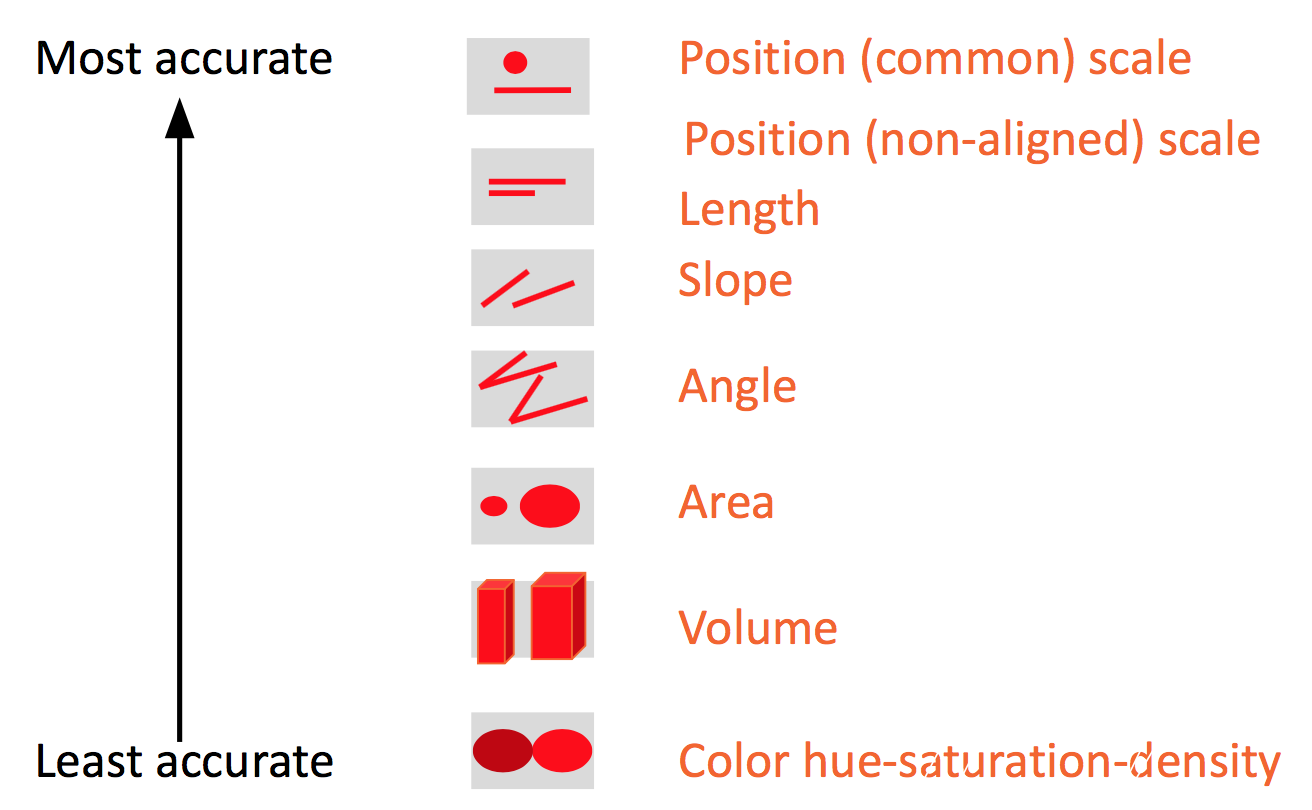
\includegraphics[width=13cm]{./img/06/magnitude}
 \caption{\label{pic:magnitude} What works and what does not.}
\end{figure}


These tasks are sorted according to how accurately people perform them.

\begin{figure}[h]%---------------FIG--------------
 \centering
 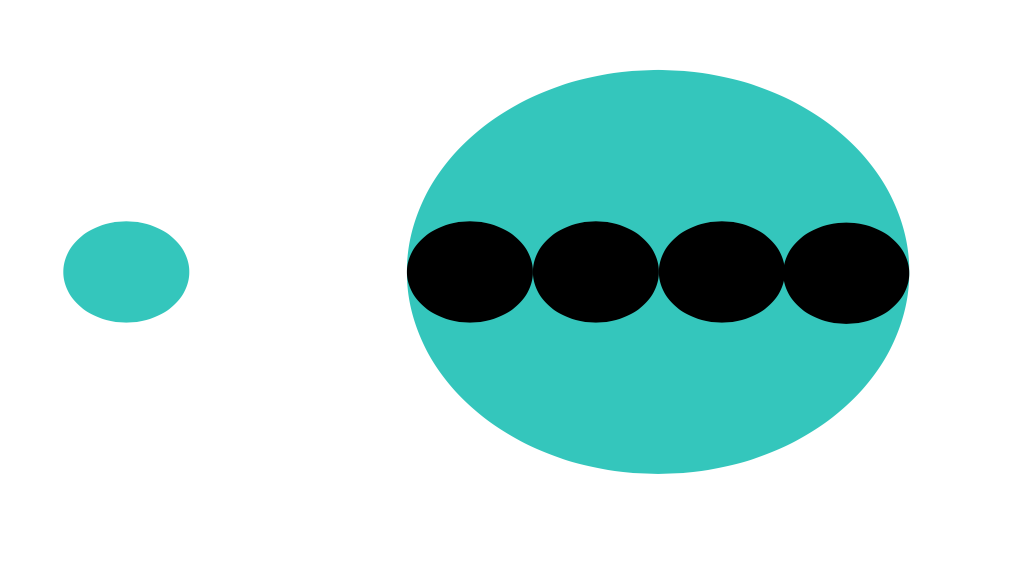
\includegraphics[width=13cm]{./img/06/area}
 \caption{\label{pic:area} How many times the \emph{little} one is included in the \emph{big} one?}
\end{figure}

\subsubsection*{Compare colors...}
Use a magnitude that allows people to easily read and interpret your data, noticeable differences are required. In 1846 the physicist Ernst Weber, defining \emph{I} as the intensity of the stimulus and \emph{S} the sensation, said that

$$\Delta S = k \frac{\Delta I}{I}.$$

It is known as the \emph{Weber's law} and reads out that a variation in the sensation is proportional to the magnitude of the original intensity of the stimulus. So as the base \emph{I} increase, we require a larger changes in  $\Delta I$ to notice the change. 

\subsubsection*{...And choose them}

Choose colors based on the information you want to convey:

\begin{itemize}
\item \emph{Sequential}: colors can be ordered from low to high (Figure \ref{pic:sequential})
\item \emph{Diverging}: two sequential schemes extended out from a critical midpoint value (Figure \ref{pic:diverging})
\item \emph{Categorical}: Lots of contrasts between each adjacent color (Figure \ref{pic:sequential})
\end{itemize}

\begin{figure}[H]%---------------FIG--------------
 \centering
 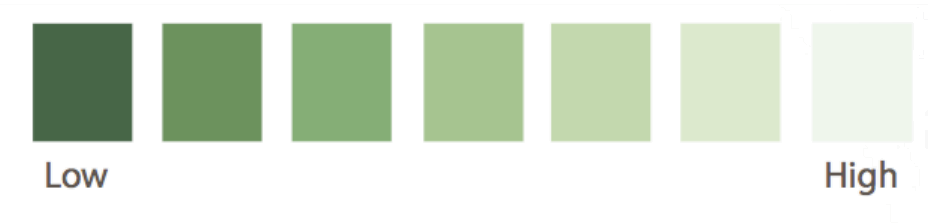
\includegraphics[width=13cm]{./img/06/sequential}
 \caption{\label{pic:sequential} Example of sequential colors.}
\end{figure}


\begin{figure}[H]%---------------FIG--------------
 \centering
 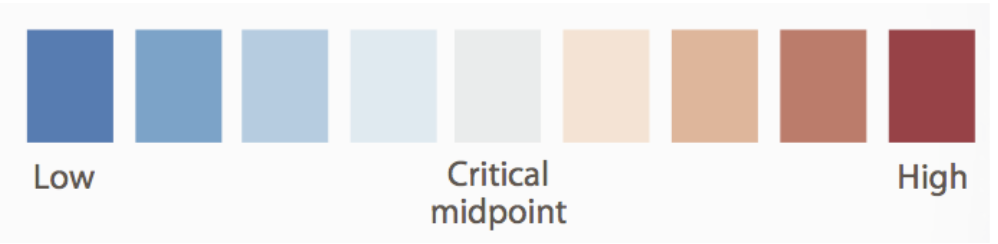
\includegraphics[width=13cm]{./img/06/diverging}
 \caption{\label{pic:diverging} Example of diverging colors.}
\end{figure}

\begin{figure}[H]%---------------FIG--------------
 \centering
 
\includegraphics[width=13cm]{./img/06/categorical}
 \caption{\label{pic:categorical} Example of categorical colors.}
\end{figure}

The usage of these tools depends on what you what to show. Anyway there are several \href{http://colorbrewer2.org/#type=sequential\&scheme=BuGn\&n=3}{online} sources that can help you to choose the color scheme according to your purpose.

\subsection*{Use Structure}

In 1912 Gestalt outlined principles that describe how our mind organizes individual visual elements into groups, to make sense of the entire visual. When designing a visual, these principles can be used to highlight patterns that are important to us, and downplay other patterns. The Figure  illustrates the \href{http://www.fusioncharts.com/blog/2014/03/how-to-use-the-gestalt-principles-for-visual-storytelling-podv/}{principles of Gestalt} which is relevant to visualization (Figure \ref{pic:gestalt}). Do not concentrate too much information, less is more!

\begin{figure}[H]%---------------FIG--------------
 \centering
 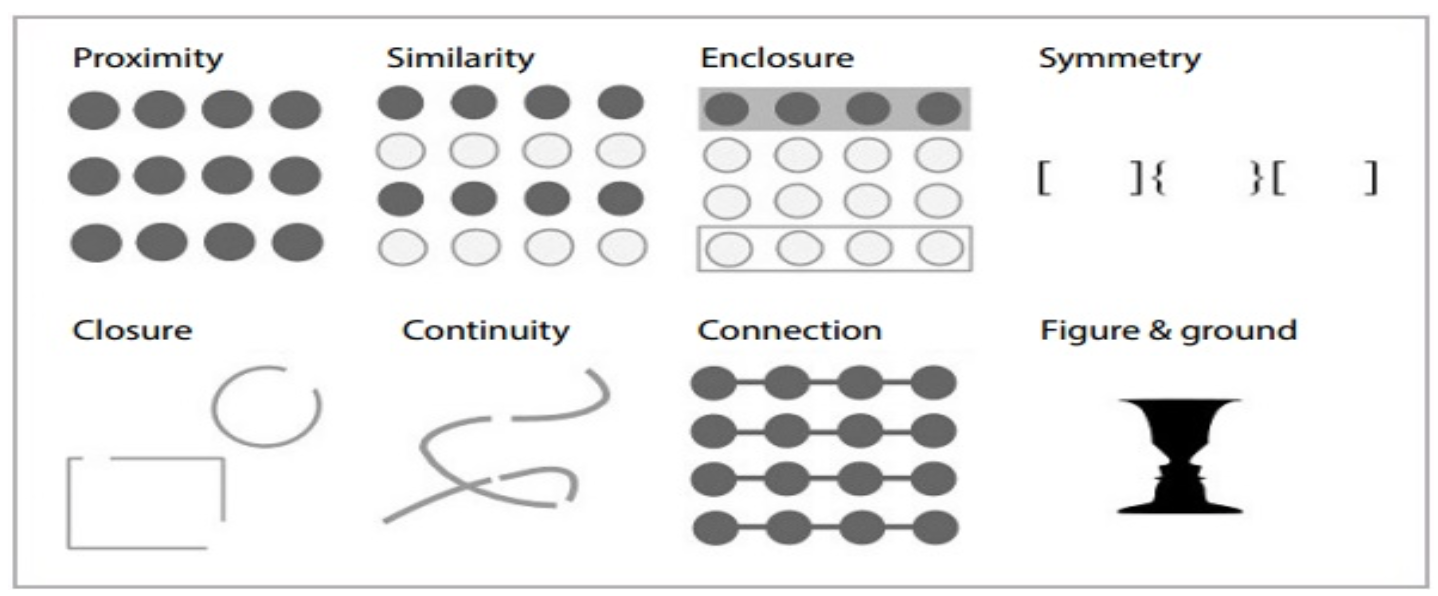
\includegraphics[width=13cm]{./img/06/gestalt}
 \caption{\label{pic:gestalt} Gestalt's principles.}
\end{figure}

Here is what we notice from each of the illustrations [\href{http://www.fusioncharts.com/blog/2014/03/how-to-use-the-gestalt-principles-for-visual-storytelling-podv/}{principles of Gestalt}]:

\begin{itemize}

\item \emph{Proximity}: we see three rows of dots instead of four columns of dots because they are closer horizontally than vertically.
\item \emph{Similarity}: we see similar-looking objects as part of the same group.
\item \emph{Enclosure}: we group the first four and last four dots as two rows instead of eight dots.
\item \emph{Symmetry}:we see three pairs of symmetrical brackets rather than six individual brackets.
\item \emph{Closure}: we automatically close the square and circle instead of seeing three disconnected paths.
\item \emph{Continuity}: we see one continuous path instead of three arbitrary ones.
\item \emph{Connection}: we group the connected dots as belonging to the same group.
\item \emph{Figure \& ground}: we either notice the two faces, or the vase. Whichever we notice becomes the figure, and the other the ground

\end{itemize}

These principles allow us to perform many tasks such as reduce the noise from charts, choose the ideal aspect ratio, and show relationships between elements more clearly. Let's look at a dashboard, and see these principles in action.

\subsection*{How to select the right chart}

The flowchart below can be helpful to understand the most suitable chart for your purpose.

\begin{figure}[H]%---------------FIG--------------
 \centering
 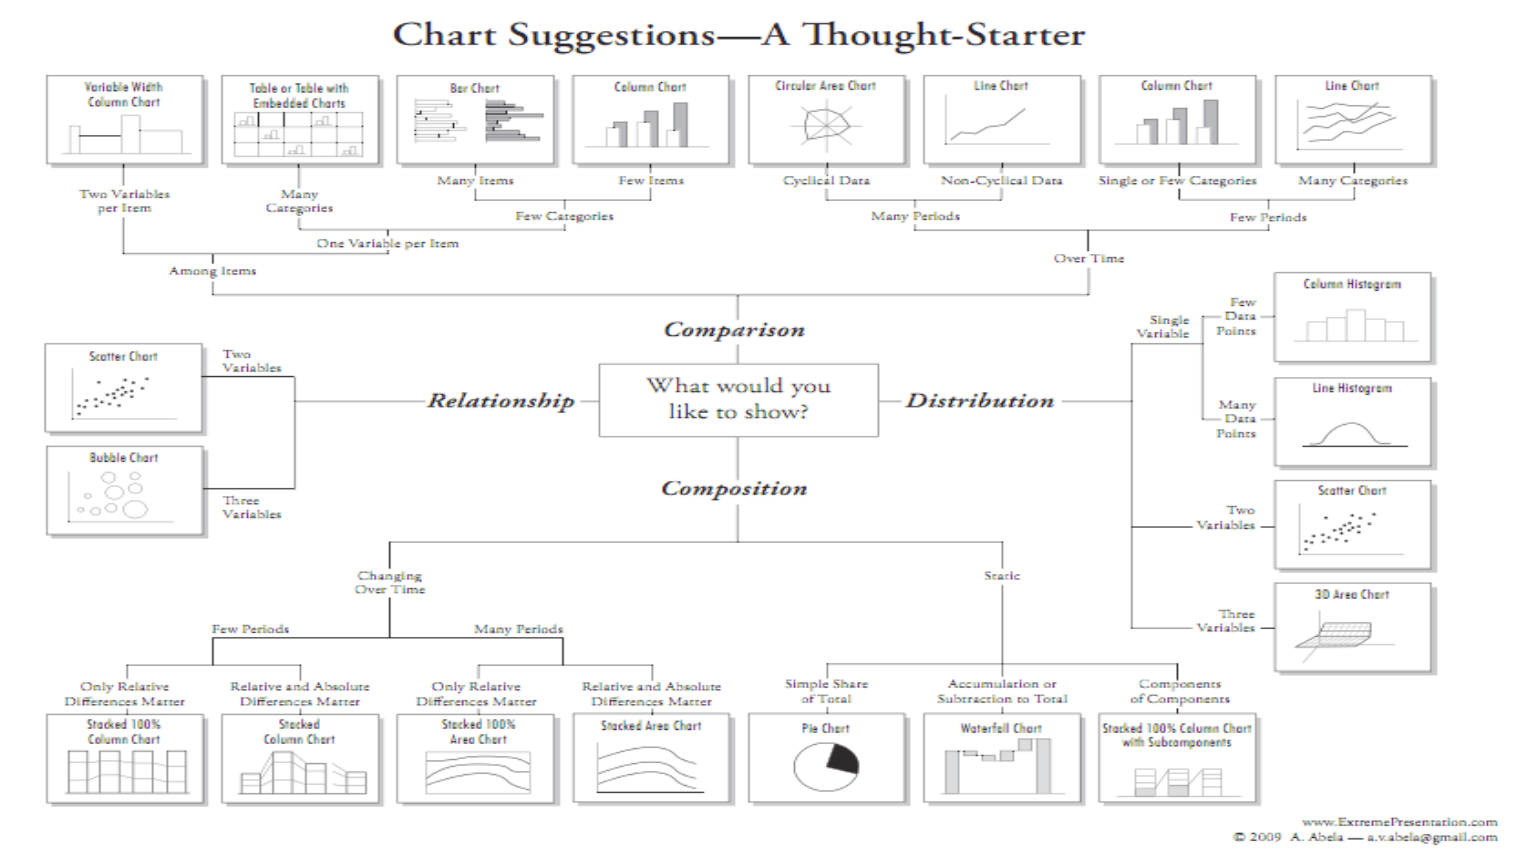
\includegraphics[width=13cm]{./img/06/flow_chart}
 \caption{\label{pic:flow_chart} Make your choice.}
\end{figure}

Instead of using the chart, you can also find sources, like \href{http://www.juiceanalytics.com}{\emph{Juice Analytics}}, that let you choose interactively, means some filters, the best chart according to your necessities.

\subsection{Interactive toolkits}

\begin{itemize}
\item \href{https://d3js.org}{\texttt{D3}} is, without doubt, the most widely used interactive visualization framework, developed around 2011 by Jeff Heer, Mike Bostock and Vadim Ogievetsky. \emph{Notes from the authors}: D3 is intentionally a low-level system. During the early design of D3, we even referred to it as a "visualization kernel" rather than a "toolkit" or "framework";

\item \texttt{Vega} is a \emph{visualization grammar} developed on top of \texttt{d3.js}. It specifies graphics in \texttt{JSON} format;

\item \href{https://vega.github.io/vega/}{\texttt{Vincent}} is a Python-to-Vega translator;

\item \href{http://bokeh.pydata.org/en/latest/}{\texttt{Bokeh}} is an independent Viz library focused more heavily on big data visualization. Has both \texttt{Python} and \texttt{Scala} bindings; 

\end{itemize}

\clearpage
% !TEX root = ../notes.tex

% ================  (Interactive) Visualization ==============

\section{Supervised Learning}

%=============================================
\subsection{Introduction to Machine Learning}

{\bf Machine Learning} is an extended field characterized by many facets. The  \href{https://en.wikipedia.org/wiki/Arthur\_Samuel}{Arthur Samuel}'s definition can be considered the most meaningful one: ``{\it Field of study that gives computers the ability to learn without being explicitly programmed.}''. The aim of \emph{Machine Learning} is to model into a computer the learning and adapting procedures that characterize the human way of thinking and processing information. Merely, the idea behind is to use computers to apply statistical and optimization algorithms to \emph{automatically} identify pattern in data and/or classify them. 

To get an idea of what \emph{Machine Learning} does and consists of, take a look at a \href{http://www.r2d3.us/visual-intro-to-machine-learning-part-1/}{beautiful introduction to Machine Learning}. In order to capture the essence of this subject, it speaks more than thousand words . 

In the end, according to a reductive point of view, we may simply say that Machine Learning is born because we are \textbf{lazy} and we let the machine do the ``work'' for us. 
\\\\
\emph{Machine Learning} is based on the definition of algorithms that allows the aforementioned procedures. Those algorithms can be distinguished either by the \emph{learning style} (Supervised vs Unsupervised vs Semi-Supervised learning) or by their \emph{similarity}. 

In the next part of this chapter, we first give an introduction to \emph{Supervised} and \emph{Unsupervised} learning and then we go deeper into \emph{Supervised Learning}. If you want to become a Machine Learning Master, you should have a look \href{http://machinelearningmastery.com/}{here}.

%=============================================
\subsubsection{Different aspects of Machine Learning} 

When we apply a \emph{Machine Learning} method, one on the thing that we are mostly interested in is getting good predictions. This is not the only important aspect of the Machine Learning methods though. 

The following list rough out some very important aspects for these methods:

\begin{itemize}
\item \textbf{Predictive accuracy}: we want our model to return correct result;
\item \textbf{Speed and scalability}: the model should be efficient in order to be easily applied
  \begin{itemize}
   \item Time to build the model
   \item Time to use the model
   \item In memory vs Disk processing
  \end{itemize}
\item \textbf{Robustness}: the method should not be too sensitive
  \begin{itemize}
   \item Handling noise
   \item Handling outliers
   \item Handling missing values
  \end{itemize}
\item \textbf{Interpretability}
  \begin{itemize}
   \item Understand the model and its decisions (\emph{black box} vs {white box})
   \item Compactness of the model
  \end{itemize}
\end{itemize}

%=============================================
\subsubsection{Supervised vs Unsupervised Learning}

In Table \ref{tab:sup-unsup} we outline some differences/similarities between \emph{Supervised} and \emph{Unsupervised} learning. 

The main difference to remark is that for \emph{Supervised} learning, we use a \emph{training} data with \textbf{known} labels and we test it on a\emph{test} data \textbf{without} labels. For \emph{Unsupervised} learning we do not have any labels. We are just trying to simplify/cluster the samples.

\begin{table}[h!]
  \centering
  \begin{tabular}{m{2cm}||m{5.5cm}|m{5.5cm}}
    & \textbf{Supervised} & \textbf{Unsupervised} \\ \hline\hline
    \textbf{Variables} & Samples $X$ and labels $y$ & Samples $X$ \\ \hline
    \textbf{Learning} & Function $y = f(X)$ relate samples and labels. We would like to ``learn'' $f$ and evaluate it on new data. & We want to compute a function $y = f(X)$ to give a \emph{simpler} representation of the samples X. \\ \hline
    \textbf{Discrete \newline labels} & {\bf Classification} & {\bf Clustering} \\ \hline
    \textbf{Continuous labels} & Regression & Matrix factorization, Kalman filtering, Unsupervised neural networks \\ \hline 
    \text{Examples} & 
	      $\bullet$ Is this image a cat, dog, car, house? \newline
	      $\bullet$ How would this user score that restaurant? \newline
	      $\bullet$ Is this email spam? \newline
	      $\bullet$ Is this blob a supernova?
	     &
	      $\bullet$ Cluster some hand-written digit data into 10 classes. \newline
	      $\bullet$ What are the top 20 topics in Twitter right now? \newline
	      $\bullet$ Find and cluster distinct accents of people in Lausanne
            \\ \hline
    \textbf{Techniques} & 
	      $\bullet$ k Nearest Neighbors \newline
	      $\bullet$ Na\"ive Bayes \newline
	      $\bullet$ Linear + Logistic Regression \newline
	      $\bullet$ Support Vector Machines \newline
	      $\bullet$ Random Forests \newline
	      $\bullet$ Neural Networks
	    &
	      $\bullet$ Clustering \newline
	      $\bullet$ Topic Models \newline
	      $\bullet$ Hidden Markov Models
	    \\ \hline
  \end{tabular}
  \label{tab:sup-unsup}
  \caption{Summary of the differences between Supervised and Unsupervised learning.}
\end{table}

%=============================================
\subsection{More details on Supervised Learning}

%=============================================
\subsubsection{Predicting from Samples}

The \textbf{samples} are, most of the time, subsets of an infinite population. We are interested in a model that can {\bf describe the whole population}, but since we only have access to a \emph{sample} of it, it is not possible. Therefore we train on a training sample $D$ and we denote the model found by $f_D(X)$, $X$ being the features.
Most of the datasets are \textbf{samples} from an infinite population, \emph{i.e.} a subset of an \textbf{infinite} dataset. We would like to model the \textbf{whole population}, but only have access to a sample of it. So, we train on a training sample called $D$ and we denote the model as $f_D(X)$ where $X$ are the features and $y=f_D(X)$ the predictions.

%=============================================
\subsubsection{Bias and Variance}

The data-generated model $f_D(X)$ is a \textbf{statistical estimate} of the true function $f(X)$ (function working for the whole population). Therefore the model is subject to bias and variance. 
\\
The \textbf{Bias} is defined as the \emph{expected difference} between the prediction of a model $f_D(X)$ and the true labels $y$:
\[
 \textrm{Bias} = \mathbb{E}\left[ f_D(X)-y\right]
\]
\\
The \textbf{Variance} is defined as:
\[
 \textrm{Variance} = \mathbb{E}\left[\left(f_D(X) - \overline{f}(X)\right)^2\right]
\]
where $\overline{f}(X) = \mathbb{E}\left[f_D(X)\right]$ being the average prediction on X.

Bias and Variance are very useful to understand if you are doing something wrong. Thus, it is important to understand what you are doing and not just applying ``black-boxed'' algorithms.

\subsubsection*{ Trade-off between Bias and Variance}

The \href{http://scott.fortmann-roe.com/docs/BiasVariance.html}{tradeoff between bias and variance} is due to model complexity, see Figure \ref{fig:simple_complex}.
\begin{itemize}
 \item \textbf{Complex models}: Many parameters, usually lower bias (the model is close to the model that generates the data) but higher variance (the predictions have high variability). It leads to the risk of overfitting. Merely, this kind of models describe well the sample population, likely they do not represent well the entire population though.
 \item \textbf{Simple models}: Few parameters, higher bias (far from the true model) but lower variance (less variability among predictions), It may ends up with the underfitting.
\end{itemize}
\begin{figure}[H] %----------- Graph ---------------------
\centerline{
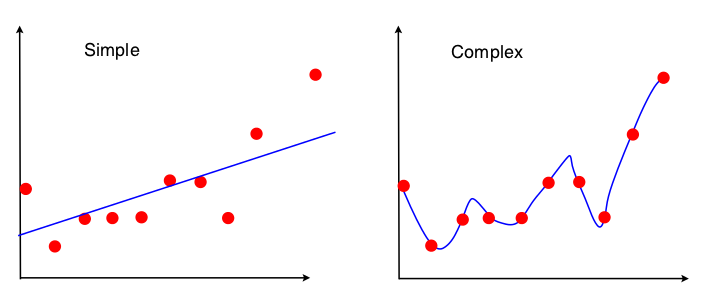
\includegraphics[width=13cm]{img/07/simple_complex}
}
\caption{\label{fig:simple_complex} 
Illustrations of a simple model and a complex model on the same data.
}
\end{figure}


For example, a linear model can only fit a straight line. A high degree polynomial can fit complex curves. Therefore this polynomial will work very well with the samples but not that well with the whole population. Thus a high variance is expected.
\\\\
In order to take into account this trade-off, we introduce the total expected error is 
\[
 \textrm{Bias}^2 + \textrm{Variance}
\]
This error {\bf balance} the contributions of the variance and the bias. 

\begin{figure}[H] %----------- Graph ---------------------
\centerline{
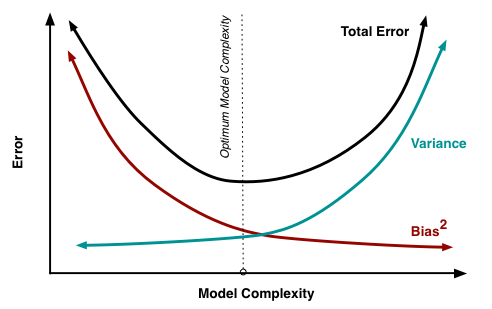
\includegraphics[width=10cm]{img/07/biasvariance}
}
\caption{\label{BV} 
Illustration of the model complexity and the Bias Variance tradeoff. The optimum model complexity is when the total error is minimized.
}
\end{figure}
When the Bias and the Variance are unbalanced, we use the terms:
\begin{itemize}
 \item {\bf overfitting} when the \emph{Variance} strongly dominates. (Too much variation between models. Hence, the model does not work well on new data)
 \item {\bf underfitting} when the \emph{Bias} strongly dominates. (The models do not fitting the data well enough)
\end{itemize}


%=============================================
\subsection{k-Nearest Neighbors}

The kNN algorithm is a well known method used for classification and regression. Given a  query item, the idea of the kNN algorithm is to find the \emph{k} nearest neighbors (\emph{k} closest matches) using a specific metric. Once we found them, we label the item such that it corresponds to the most frequent label in the neighbors. Figure \ref{fig:knn} shows an example with cats and other animals.

\begin{figure}[H] %----------- Graph ---------------------
\centerline{
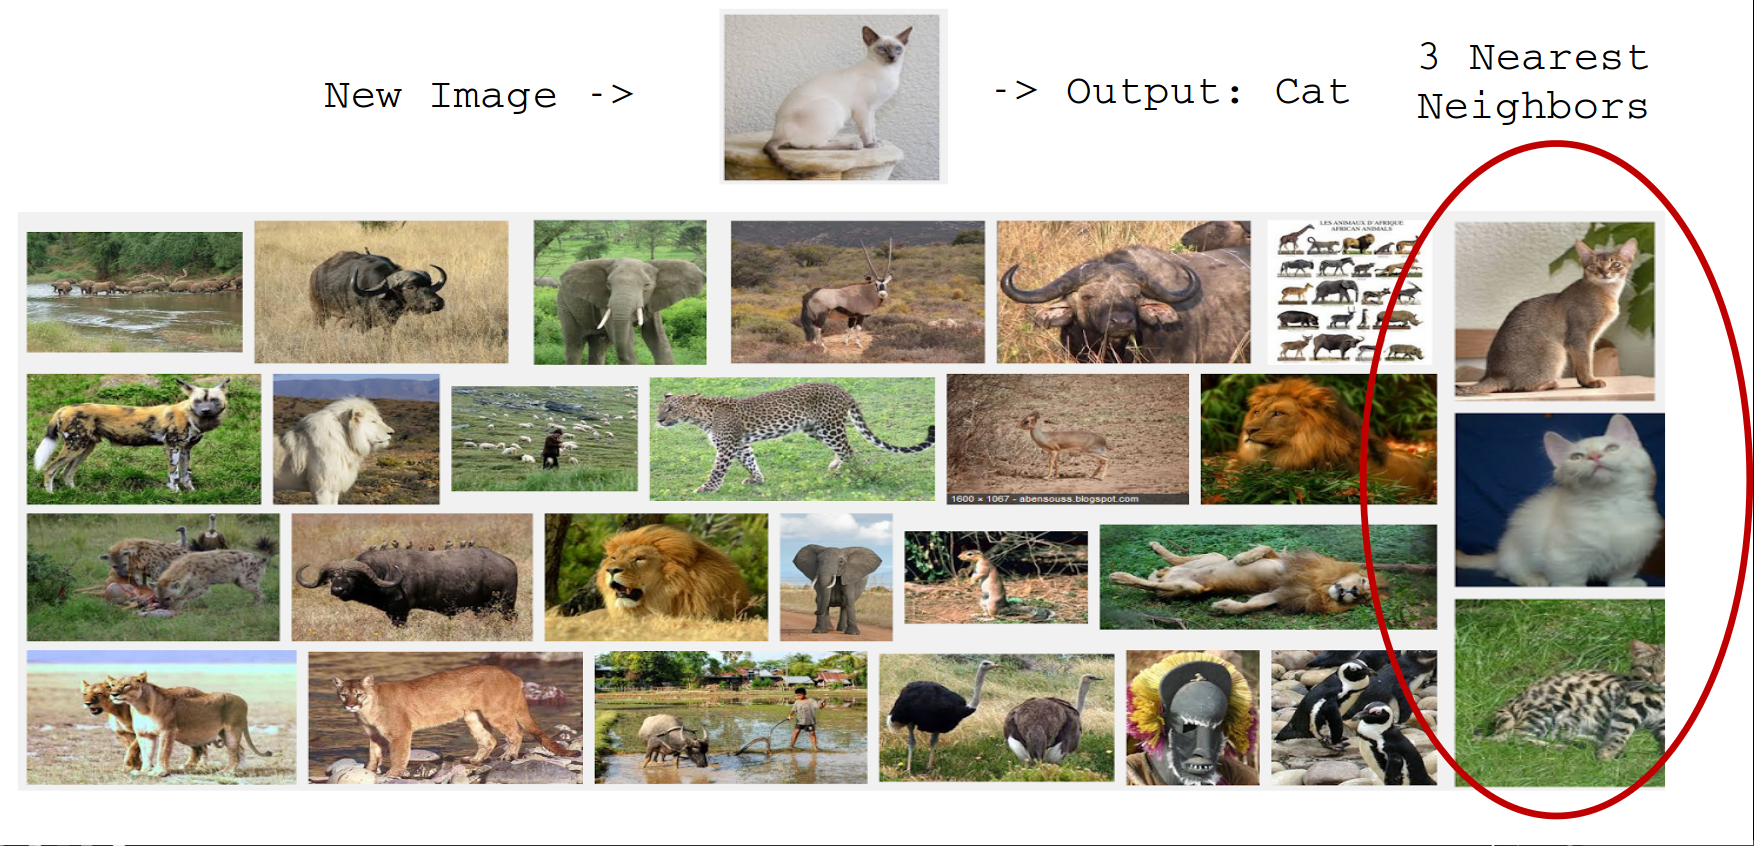
\includegraphics[width=13cm]{img/07/knn}
}
\caption{\label{fig:knn} 
Illustration of the kNN algorithm.
}
\end{figure}

However, this very simple algorithm has one issue: the Data {\bf is} the Model. This implies:
\begin{itemize}
 \item No training needed.
 \item The accuracy generally improves with more data.
 \item Matching is simple and fairly fast if data fits in memory. (Can be run off disk)
\end{itemize}
Normally, the only parameter is $k$, the number of neighbors. But two other choices are important:
\begin{itemize}
 \item Weighting of neighbors (e.g. inverse distance)
 \item Similarity metric.
\end{itemize}

%=============================================
\subsubsection{kNN Flavors}
The kNN algorithm can be used both for regression and classification. Table \ref{tab:knn} gives the similarities/differences of the kNN algorithm for regression and classification.
\begin{table}[h!]
 \centering
 \begin{tabular}{p{7cm}|p{7cm}}
  \textbf{Classification} & \textbf{Regression} \\ \hline \hline
  The model is $y=f(X)$ where $y$ is from a discrete set (labels). & The model is $y=f(X)$ where $y$ is a real value. \\ \hline
  Given $X$, we compute $y$ being the majority vote of the k nearest neighbors. & Given $X$, we compute $y$ being the average value of the k nearest neighbors. \\ \hline
  We can also use a weighted vote of the neighbors. & We can also use a weighted average of the neighbors.
 \end{tabular}
 \label{tab:knn}
 \caption{kNN algorithm used for classification and regression: Differences and similarities. Usually, the weight function is the inverse distance. 
}
\end{table}

%=============================================
\subsubsection{kNN distance measures}
For the kNN algorithm, we need to use a distance between the neighbors. The choice of the distance function can be very different depending on what you are looking for. We give here some examples:
\begin{description}
 \item[Euclidean distance]: Simple and fast to compute.
 \[
  d(x,y) = ||x-y||
 \]

 \item[Cosine Distance]: Good for documents, images, etc.
 \[
  d(x,y) = 1- \frac{x\cdot y}{||x||||y||}
 \]

 \item[Jaccard Distance]: For set data
 \[
  d(X,Y) = 1 - \frac{|X \cap Y|}{|X \cup Y|}
 \]

 \item[Hamming Distance]: For string data
 \[
  d(x,y) = \sum_{i=1}^{n} \left( x_i \neq y_i \right)
 \]
 \item[Manhattan Distance]: Coordinate-wise distance
 \[
  d)x,y) = \sum_{i=1}^n |x_i - y_i|
 \]
 \item[Edit Distance] For strings, especially genetic data. See on \href{https://en.wikipedia.org/wiki/Edit\_distance}{Wikipedia} for more information.
 \item[Mahalanobis Distance] Normalized by the sample covariance matrix -- unaffected by coordinate transformations. 
 \[
  d(x,y) = \sqrt{\left(x-y\right)^TS^{-1}\left(x-y\right)}
 \]
 where $S$ is the covariance matrix.
\end{description}

%=============================================
\subsubsection{Choosing k}

If we choose a {\bf small k}, we will see a low bias but high variance. Firgure \ref{fig:knn_k1} shows whats happens with two different samples if we choose a small k.

\begin{figure}[H] %----------- SubGraph ---------------------
\centerline{
\subfigure{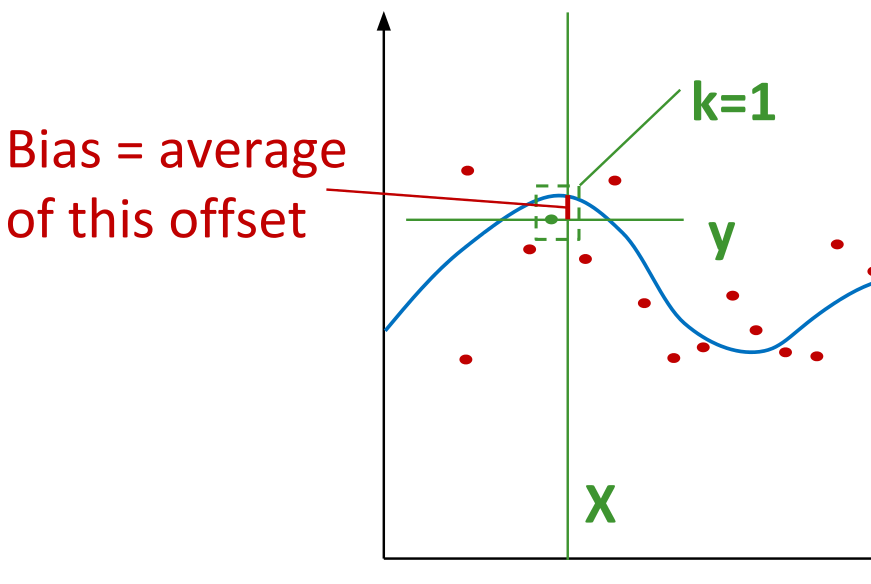
\includegraphics[width=7cm]{img/07/k1_original}}\quad
\subfigure{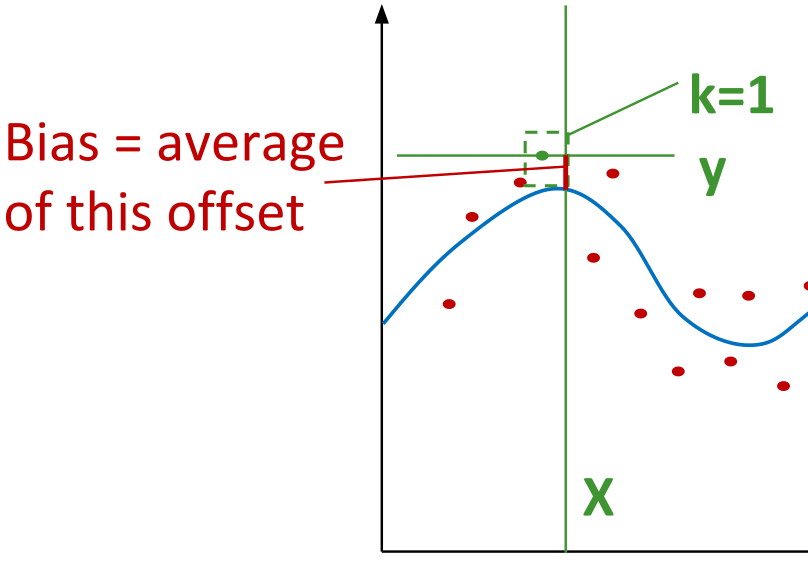
\includegraphics[width=7cm]{img/07/k1_diff}} 
}
\caption{\label{fig:knn_k1} 
Test on two different samples of the kNN algorithm with k=1.
}
\end{figure}

On the other hand if we choose a {\bf large k}, we will see a high bias but low variance. Firgure \ref{fig:knn_k8} shows whats happens with two different samples if we choose a large k.

\begin{figure}[H] %----------- SubGraph ---------------------
\centerline{
\subfigure{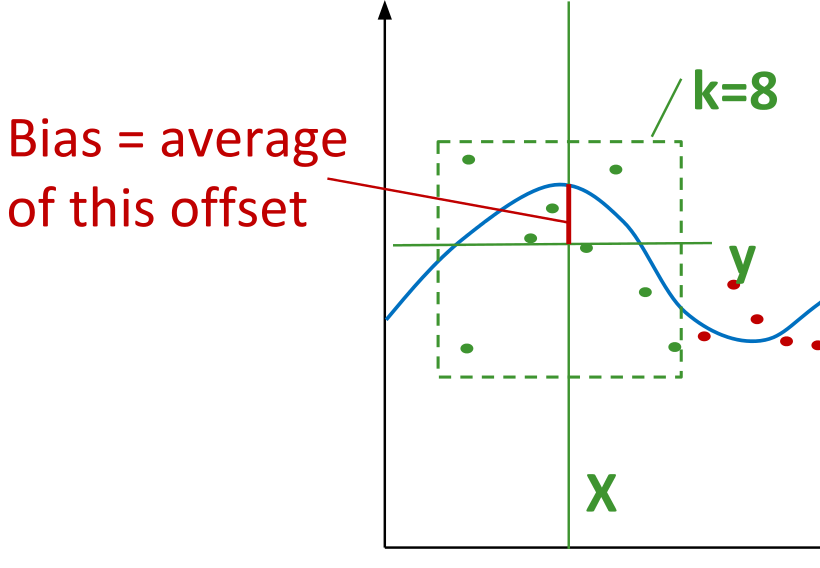
\includegraphics[width=7cm]{img/07/k8_original}}\quad
\subfigure{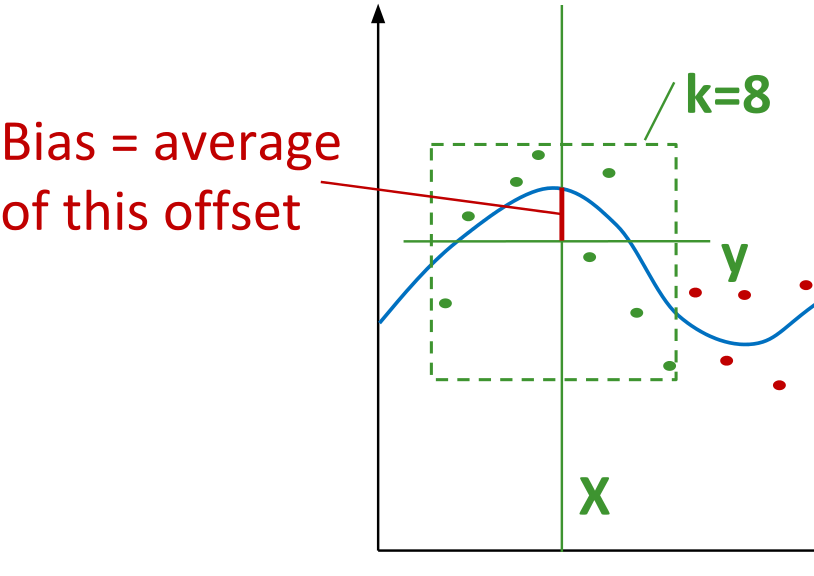
\includegraphics[width=7cm]{img/07/k8_diff}} 
}
\caption{\label{fig:knn_k8} 
Test on two different samples of the kNN algorithm with k=8.
}
\end{figure}

\subsubsection*{In practice}

\begin{description}
 \item[Use cross-validation!] Break data into train, validation and test subsets. For example, you can choose a 60-20-20 \% random split.
 \item[Predict] For each point in the validation set, predict using the k-Nearest neighbors from the training set. Measure the error rate (classification) or the squared error (regression)
 \item[Tune] Try different values of k, and use the one that gives minimum error on the validation set.
 \item[Evaluate] test on the test set to measure performance.
\end{description}

%=============================
\subsubsection{kNN and the curse of dimensionality}

The curse of dimensionality refers to phenomena that occur in high dimensions, from hundreds to millions, that do not occur in low-dimensional space. Data in high dimensions are much sparser than data in low dimensions. That means there are less points that are very close in the feature space. For example, the Euclidean distance scales as $\sqrt{N}$ with $N$ being the dimension. Thus it is quite surprising that kNN works even in high dimensions. 

Luckily data are not random points in a high-dimensional cube. They live in {\bf dense clusters} and near {\bf much lower-dimensional surfaces}. Therefore, we can reduce the feature space in many different way to see the clusters appear.

Even if the Euclidean distance between two point is large they can be very \emph{similar}. For example documents with the same few dominant words (with \href{https://en.wikipedia.org/wiki/Tf-idf}{tf-idf} weighting) are likely to be on the same topic.

\clearpage
%=============================
\subsection{Decision Tree}

Decision Tree (DT) is a basic classifier acting like a \textbf{flow-chart having the following tree structure}  :
\begin{itemize}
	\item \textbf{Decision node}: specifies a test on a single attribute
	\item \textbf{Leaf node}: indicates the value of the target attribute
	\item \textbf{Edge}: split on one attribute
	\item \textbf{Path}: a disjunction of tests to make the final decision
\end{itemize} 

It's constructed following a top-down approach in which, at each node, the data is split on one of their attribute. The prediction are obtained by following the "if-else" statement of each node and is given by the leaves , once the whole tree is traversed (Path). 
\\\\

\textbf{Accuracy} \\
Training accuracy : How many training instances can be correctly classified based on the available data? It is high when the tree is deep/large, or when there is less conflictual instances in the training instances. Never forget that higher training accuracy does not mean good generalization.
Testing accuracy: Given a number of new instances, how many of them can we correctly classify. The only way to score a DT is by counting the number of right elements it predicts on the test set, since the prediction are not "weighted" by a probability of correctness.

\begin{figure}[H] %----------- SubGraph ---------------------
\centerline{
\subfigure{\includegraphics[width=5.5cm]{img/07/DT1}}
\subfigure{\includegraphics[width=5.5cm]{img/07/DT2}} 
}
\caption{\label{DT} 
Dataset and the Decision Tree related to it.
}
\end{figure}

\textbf{Construction} (Top-down, divide-and-conquer strategy.)
\begin{enumerate}
  \item At the beginning, all the samples are attached to the root.
  \item Recursively, the (sub)sets are partitioned according to their most discriminative attribute (see section \ref{sec:selection} for the ways of selecting of the attributes).
  \item Stop when:
  \begin{itemize}
  	\item A node only contains identically labelled samples, this node becomes a leaf .
  	\item No more attributes are left for splitting, assign the most dominant label to the leaf.
  	\item No more samples left.
  	\item A depth threshold has been defined and has been reached.
  \end{itemize}
\end{enumerate}

The DT will continue to add attributes to its decision process until none are left. As it increases its precision (and then its depth), it starts over fitting the model. A threshold can be defined to stop the construction process earlier and limit this effect. 

\begin{figure}[H]%---------------FIG--------------
 \centering
 \includegraphics[width=10cm]{./img/07/bias_variance_DT.png}
 \caption{\label{pic:bias_variance_DT.} Bias and variance evolution with DT depth}
\end{figure}

\begin{center} %---------------TAB--------------
\begin{tabular} {| l | l |}
\hline
\bf Pros & \bf Cons \\ \hline
+ A first ML approach ;) & - Sensitive to small perturbation  \\
+ Can be enhanced in RF or BDT  & - Retrained from scratch when new data are coming \\
+ Simple to understand and interpret & - Tend to overfit \\
+ Requires little data preparation \\ 
\hline
\end{tabular}
\end{center}



%=============================
\subsubsection{Attribute selection}
\label{sec:selection}

A big part of the DT model creation relies on choosing the good attribute on which to split the data in each node. One way to achieve this splitting relies on the concept of entropy, which describes the disorder a system and how impactful a feature can be.

For a set $S$ with $P$ positive predictions and $N$ negative ones, its entropy is:
$$
 H(P,N)=-\frac{P}{P+N}\log_2\frac{P}{P+N}-\frac{N}{P+N}\log_2\frac{N}{P+N}
$$
Note that:
\begin{itemize}
 \item If $P \text{ or } N=0 \rightarrow H(P,N)=0$, meaning \textbf{no uncertainty at all}
 \item If $P=N \rightarrow H(P,N)=1$, meaning \textbf{maximum of uncertainty}
\end{itemize}

Entropy of the attribute $A$:
$$
H(A) = \sum_{i} \frac{P_i + N_i}{P + N} * H(P_i, N_i)
$$

Gain obtained by splitting the dataset $S$ by attribute $A$.
$$
Gain(A) = H(P, N) - H(A)
$$

The gain indicates how a split on a certain attribute will influence our data set. The lower the entropy becomes, the greater is the gain, the more \textit{organised} and \textit{certain} become the data set.

The figure \ref{pic:entropy} illustrates how the entropy of an attribute is calculated.

In order to choose how to next split $S$, we compute the gain of each attribute $A$ regarding $S$ and choose the best.

\textbf{Pruning} The construction algorithm aforementioned 	doesn't filter out noise which may lead to over fitting. In order to circumvent this disagreement the Decision tree can be \href{https://en.wikipedia.org/wiki/Pruning_(decision_trees)}{pruned}.


\begin{figure}[H]%---------------FIG--------------
 \centering
 \includegraphics[width=10cm]{./img/07/entropy.png}
 \caption{\label{pic:entropy} Example of entropy calculation.}
\end{figure}






%========================================
\subsubsection{Random Forest}

A common problem when trying to build a model is to select significant features between all the available ones. We tend to think that \textit{the more we have, the better it is}, even knowing the existence of the curse of dimensionality. 

Random Forest exploits this previous idea and tries to automatize the feature selection process by randomly selecting subsets of features.

The main idea of Random Forest algorithm is to grow an arbitrary number of \textbf{Decision Trees}, each one based on a subset of m features, randomly chosen between the total $p$. It's an example of \textbf{weak learners} seen in the Ensemble method. These weak learners have a lower bias (because of lower number of feature).

\textbf{Ensemble methods} can be compared to crowd-sourced machine learning algorithms in the sense that we use a collection of weak learners and combine their results to make a better prediction. There are several different types of ensemble methods : 
\begin{itemize}
	\item \textbf{Bagging :} Train learners in parallel on different samples of the data and then combine the results by voting/averaging for discrete/continuous outputs.
	\item \textbf{Stacking :} A first series of learners is trained on the samples, then a combiner algorithm is trained to make a final prediction using the outputs of the first series of learners.
	\item \textbf{Boosting :} (see next section)  
\end{itemize}

\begin{center} %---------------TAB--------------
\begin{tabular} {| l | l |}
\hline
\bf Pros & \bf Cons \\ \hline
+ Popular & - Not state-of-the-art  \\
+ Easy to implement & - Needs many passes over the data \\
+ Easy to parallelize & - Tend to overfit \\ 
\hline
\end{tabular}
\end{center}

%===============================
\subsubsection{Boosted Decision Trees}
Variant of Random Forests. Instead of performing the training of all DTs independently on a weak subset, train learners on the filtered outputs of other learners. The building of the ensemble is incremental where each new model instance is made to emphasize instances that previous models mis-classified. The accuracy yielded by boosting can be better than bagging but it also tends to overfit the training data. 
This is called \textbf{Boosting}. 
\begin{itemize}
\item Low variance, because of the small trees handling small numbers of features
\item Low bias, reduces by the boosting
\end{itemize}

Opposed to Random Forests that usually trains tens of medium-sized trees, Boosted Decision Trees works on smaller trees in greater numbers.

On the side of performances, even if they show good results, the big drawback of Boosted Decision Trees is their slow execution compared with the parallelized Random Forest.

%===============================
\subsubsection{About model transparency}

A recurrent argument of using Decision Tree (DT) or Random Forest (RF) in industry is their transparency compared to state-of-the-art Deep-Neural-Network (DNN) that are often "black-boxed". This argument must be carefully taken. Even if by their very nature DT are more understandable by a human than DNN, the more features and Trees we had, the more complicated it becomes and the less transparency we have even for DTs. Figure \ref{pic:RF_BT} shows the size of a common industry implementation of RF and BT where there are no more possibilities of human understanding.

\begin{figure}[H]%---------------FIG--------------
 \centering
 \includegraphics[width=10cm]{./img/07/RF_BT.png}
 \caption{\label{pic:RF_BT.} Standard size of RF and BDT implementations.
 In red: RF with big parallel DT. In green: BDT pipeline with lot of small DT}
\end{figure}


\subsection{Linear Regression}

Linear regression model produces a prediction equation:

$$
\hat{y} = \hat{\beta_0} + \sum\limits_{j=1}^p  X_j \hat{ \beta_j}
$$

or in matrix notation

$$
\hat{y} =X \hat{ \beta}
$$

Where $X = \begin{pmatrix} X_{11} & \cdots & X_{1N} \\ \vdots & \ddots &  \vdots \\ X_{M1} & \cdots & X_{MN} \end{pmatrix}$ is the input data, more precisely, rows of $X$ are distinct observations and columns of $X$ are input features.The $\hat{\beta_j}$ are the coefficients of the model. 

\paragraph{Least Squares Solution}

The most common measure of fit between the line and the data is the \href{https://en.wikipedia.org/wiki/Least_squares}{least-squares} fit because if we start from the hypothesis that the points are the addition of a line with Gaussian noise, the least squares corresponds to the maximum likelihood solution.

\paragraph{Overfitting}

A common mistake that leads to overfitting is to ignore feature selection, in fact having more features doesn't mean getting better results. Therefore it's always a good idea to carefully select features to improve model accuracy. More advanced models of regression include forms of feature control such as \href{https://en.wikipedia.org/wiki/Tikhonov_regularization}{ridge regression} or \href{https://en.wikipedia.org/wiki/Lasso_(statistics)}{Lasso regression} that include embedded regularizers.

\subsubsection{Statistic validation}

As a linear model can be evaluated for every possible existing dataset, it is not enough to compute it, but the existing of a meaningful linear relationship in the data must be determined beforehand.

\paragraph{$R^2$-value}

$R^2$-value describes how much of the total variance is reduced when we include the line as an offset. It computes the distances between the real $y$ and the predicted $\hat{y}$, and compares them with the distance between real $y$ and the mean $\bar{y}$. It's therefore a good indicator on how a line fits our data.

\begin{itemize}
\item if $R^2 = 0$, then there is no difference between the linear model and the trivial mean $\bar{y}$. Then we conclude that there is not any evidence of linear relationship in our dataset and \textbf{we cannot use the model}.
\item if $R^2 = 1$, then the data perfectly aligned on the linear regression line and \textbf{the model is perfect}.
\end{itemize}

\begin{figure}[H]%---------------FIG--------------
 \centering
 \includegraphics[width=10cm]{./img/07/r_2.png}
 \caption{\label{pic:r_2} Graphical meaning of $R^2$-value.}
\end{figure}


\paragraph{p-value}

From the Distribution of Fisher (F-Distribution) we can derive a p-value which is, as usual, the probability that the observed data validates the null hypothesis which is, in our case, the hypothesis \textit{that there is no linear relationship in the data}. For $p < 0.05$ we conclude, as usual, that it is very unlikely that the data were produced by the null hypothesis and we then accept the hypothesis \textit{the data follows a linear relationship}.















\clearpage

\end{document} %%%% THE END %%%%


% Note: 
% To directly compute the main document when working on a chapter.tex, past the following
% line at the very beginning of the file
 
% !TEX root = ../notes.tex